\chapter{RELATED WORK}
\label{ch:related-work}

\sepfootnotecontent{fn:speedrun-com-re4-guides}{Footnote: Speedrun.com Resident Evil 4 Guides}

\sepfootnotecontent{fn:beat-em-up}{Footnote: What are beat 'em up games}

\section{Overview}
% * ======================================================================
% * ======================================================================
% *  OVERVIEW
% * ======================================================================
% * ======================================================================

% Review of previous research on adaptive systems and DDA
% Summary: Player Experience, Challenge, Learning Curve
% -----------------------------
% Understand the impact of difficulty in player experience
% How difficulty can be a detrimental factor or assist player improvement
% Identify problems with fixed difficulty curves
In this chapter, we perform a review of previous research and literature related to adaptive systems and dynamic difficulty. We begin by exploring literature regarding player experience and the concepts that define game difficulty, to understand the impact of difficulty in player experience. We attempt to understand how difficulty can be a detrimental factor or used as a support tool for players to learn, understand and improve upon the use of game mechanics and systems. We identify the problems with fixed difficulty curves, where the game provides a limited set of options for players to define their expected challenge level within the experience of a game. 

% Summary: Player Modelling
% -----------------------------
% Early models, concepts and terminology for dynamic adaptation
% Concepts: player models, profile, performance and preferences
% Metrics and adjustments
We proceed by studying the early models developed to address the issue of dynamically adapting a game to different players, as well as the concepts and terminology for the implementation of such models. First, we understand the concept of player models, where player behavior is monitored to create data sets that can represent player \emph{profile}, \emph{performance} and \emph{preferences}. We relate player models to the concepts of \emph{metrics} and \emph{adjustments}, where player models are used as input for dynamic adaptation game content to satisfy contextual player needs.

% Summary: Adaptive Systems in Research
% -----------------------------
% Review of AGS methods
% Understand how AGS can be used to alleviate steep learning curve
% Accommodate beginner players to challenge in difficult video games 
We proceed by reviewing previous implementations for AGS (Adaptive Game Systems), which propose to enhance player experience based on player profile, performance and preferences. We attempt to understand how AGS can be used to alleviate the steep learning curve of highly challenging games, accommodating the skill level of beginner players to the level of challenge proposed by game designers in difficult video games.

% DDA implementations: probability-based, affect-based, learning-based
% Identify positive and negative aspects of each implementation
% Focus on impact on player experience and feasibility in game development
We review multiple DDA (Dynamic Difficulty Adjustment) implementation methods, such as \emph{probability-based}, \emph{affect-based} and \emph{learning-based} adjustments. We identify the positive and negative aspects with each method regarding their impact on player experience, as well as how they can be adapted to the development of commercial games.

% Summary: Adaptive Systems in Commercial Games
% -------------------------------
% Evaluate adaptive systems in commercial games
% Understand impact of solutions in most successful games
% Explain solutions in detail, verifying positive & negative aspects
We also evaluate some of the efforts in adaptivity in commercial games, analyzing their positive and negative effects. We attempt to understand the impact of solutions implemented in some of the most successful commercial games in the last decades. We analyze representative examples for the implementation of each dynamic adaptation method in detail, verifying the positive and negative aspects of each proposed solution.

% Summary: Conclusions
% -----------------------------
% Comparative tables for adaptive concepts
% Analyze general positive and negative aspects
% Synthesize general guidelines on what should be pursued or avoided
% Understand what can be improved or explored 
We conclude by summarizing the terminology and concepts that relate to adaptive systems, and relating such concepts to the analyzed examples in research and commercial solutions.  We analyze the general positive and negative aspects that involve each type of dynamic adjustment, and synthesize general guidelines on what should be pursued or avoided in adaptive systems.

\section{Domain Context and Terminology}
% * ======================================================================
% * ======================================================================
% *  DOMAIN CONTEXT AND TERMINOLOGY
% * ======================================================================
% * ======================================================================

The objective of this work is to create a reliable system that is able to improve experience for any player, regardless of their skill level and expected challenge towards a game. To understand how to improve player experience, we must first define what constitutes it. In this section, we identify the components that constitute player experience based on previous research in usability applied to the specific context of games. 

We attempt to extract concrete, functional features from the subjective term \emph{experience}, and translate these features into tools to design a proper challenge for the player, as well as to avoid mistakes and misconceptions on level design. To perform such a task, we analyze the impact of difficulty in games and its boundaries by reviewing literature on the psychology of player enjoyment. We review why the correct level of challenge can contribute to increasing levels of immersion and the overall positive experience of a player.

\subsection{Definition of Player Experience}

Computer software is commonly developed with the objective of allowing an user to execute a set of tasks, determined by a clear objective and in a specific context \cite{ARTICLE_FromUsabilityToPlayability}. One of the early endeavors in the field of HCI (Human-Computer Interaction) was the efficiency of performing the \emph{task} to ensure a product's instrumental value \cite{ARTICLE_UserExperienceAResearchAgenda}. In this line of thought, users of an application should ideally perform tasks without thinking about the application. 

Research on the interaction between people and systems in the field of HCI led to the concept of \emph{usability}, defined by \cite{ISO_ISO92411} as:

\begin{quotation}
"The extent to which a system, product or service can be used by specified users to achieve specified goals with effectiveness, efficiency and satisfaction in a specified context of use."
\end{quotation}

This definition specifies the three qualities of a usable product: \emph{effectiveness}, \emph{efficiency} and \emph{satisfaction}. We argue that while effectiveness and efficiency can be related to productivity,  satisfaction may not be fulfilled solely by productivity. For instance, an user might feel dissatisfied with the audiovisual components of an application such as its interface, even though the application perfectly satisfies the purpose of assisting in the completion of tasks efficiently.

In \citep{ARTICLE_UserExperienceAResearchAgenda}, we learn that early works on usability expressed that productivity is not primary, but only a contributor to \emph{User Experience}. The term "user experience" does not have a standard definition, but can be seen as how people interact with products and the resulting experience and emotions \cite{ARTICLE_UnderstandingExperience}. The experience is therefore a consequence of: the user's state, such as their emotions and needs; the characteristics of the product, such as usability and audiovisual aspects and the context of use, such as the environment and date.

According to \cite{ARTICLE_FromUsabilityToPlayability}, the concept of \emph{usability} is not sufficient to fully describe UX (User Experience) in relation to Video Games. The authors argue that video games are a specific type of interactive system used for leisure purposes. Thus, when evaluating quality not only instrumental values should be considered, but also non-instrumental values such as storytelling, visuals and character design. The author also introduces the concept of \emph{Player Experience}, a specialization of UX that emphasizes the specific properties of experience in games.

The author explains that Player Experience is characterized by \emph{Playability}, a concept based on Usability but with different meanings in the video game context. The proposed definition of \emph{Playability} by \cite{ARTICLE_FromUsabilityToPlayability} resembles the original Usability definition, but emphasizes the user-centric perspective and the satisfaction property:

\begin{quotation}
"Playability represents the degree to which specified users can achieve specified goals with effectiveness, efficiency and specially satisfaction and fun in a playable context of use."
\end{quotation}

This definition is further explained when the author introduces a set of seven attributes that compose Playability: \emph{Satisfaction}, \emph{Learnability}, \emph{Effectiveness}, \emph{Immersion}, \emph{Motivation}, \emph{Emotion} and \emph{Socialization}. The concepts of effectiveness and satisfaction remain present in this definition, but are specialized or complemented. Efficiency is specified as \emph{learnability} and \emph{immersion}, and the satisfaction aspect is complemented by\emph{emotion}, \emph{motivation} and \emph{socialization} to define a set of user-centred attributes. Since this work focuses on a single-player environment, we will discuss the first six attributes and evaluate which of them can be manipulated by a reliable system through AGT.

\emph{Satisfaction} is the degree of enjoyment derived from playing, characterized by \emph{fun}, \emph{disappointment} and \emph{attractiveness}. Fun is classified as the ability of a game to entertain the player whether through challenge, curiosity or competition. Disappointment refers to the feeling of disappointment of the player in relation to a game. Attractiveness encompasses any functional or aesthetic features that increases the pleasure of play such as realistic visuals, exceptional character design or interesting systems.

\emph{Learnability} is defined as the player's capacity to understand the game systems and improve their level of proficiency in relation to the game. It is categorized by \emph{Game Knowledge}, \emph{Difficulty}, \emph{Frustration}, \emph{Speed} and \emph{Discovery}. In this context, Game Knowledge refers to the player's prior expertise to the game's mechanics and environment, and influences how the player is affected by the \emph{learning curve} [FN]. Skill can be identified in the player's cognitive aspects such as strategic and analytic decision-making, or interactive aspects with efficient usage of game mechanics.

\emph{Difficulty} relates to the challenge perceived by a player in relation to their skill. The degree of difficulty can either encourage a player to improve by learning how to play or cause frustration. Frustration relates to the feeling of uneasiness when failing to complete a particular objective and is often part of the learning process. Speed refers to the pace in which new concepts are presented to players and affects the game's learning curve. Discovery refers to the techniques employed by the game to help players assimilate game content such as interfaces or level design, and directly affects the learning curve.

\emph{Effectiveness} refers to the resources necessary to entertain players, determined by \emph{Completion} and \emph{Structuring}. Completion is related to the overall percentage of players that feel motivated to reach the game's final goal. Structuring emphasizes the locality of content as when, where and how gameplay elements appear in the game. For instance, the placement of enemies and level geometry will contribute to how the player perceives and performs an objective, indirectly affecting the learning process.

\emph{Immersion} depicts the capacity of a game to be believable in a way that the player becomes involved, losing their awareness of surroundings and sense of time. The \emph{immersion} factor can be determined by \emph{Conscious Awareness}, \emph{Absorption}, \emph{Realism} and \emph{Dexterity}. Conscious Awareness is the degree to which a player is aware of the in-game outcomes of their actions, so that they can effectively plan and execute according to a situation. Absorption refers to the level of focus of a player has to a game in a given moment, and is inversely proportional to the level of focus to their real world surroundings. Realism depicts how the game's presentation influences the ease of player absorption, relying in game characteristics such as controls and game atmosphere. Dexterity relates to the ease of a player handling the game's controls and systems, so that performing in-game actions is natural and effortless.

\emph{Motivation} is the group of attributes that compel the player to perform one or various in-game actions, defined by \emph{Encouragement}, \emph{Curiosity} and \emph{Self-Improvement}. Encouragement is the level of confidence felt by a player when facing unexplored challenges. Curiosity is the degree to which a player is interested in interacting with new elements. Self-Improvement is the process of ability development and happens any time a player must overcome a challenge that is more difficult than their skill level. 

\emph{Emotion} refers to involuntary player responses to the cognitive stimulus of a video game, defined by \emph{Reaction}, \emph{Conduct} and \emph{Sensory Appeal}. Reaction consists of the emotional response of a player in relation to a series of in-game events. Conduct is the ability of a game to conduct a player through a proposed range of emotions caused by different stimuli. Sensory Appeal denotes how interesting a game is in the aesthetic perspective using different sensory channels. For instance, a game with realistic graphics and sound effects might appeal to the audiovisual sensory channel of players.

The definition of \emph{Playability} proposed by \citet{ARTICLE_FromUsabilityToPlayability} defined several attributes that categorize the characteristics of a player, the resources employed by a game and how different game aspects are able to affect a player. We argue that one of the concepts that is most frequently discussed in this work is that of  \emph{Challenge}. If challenge is presented poorly, the player might feel frustrated and discouraged to self-improve. Thus, the level of challenge must not deviate exceedingly from the level of skill by a player. In another perspective, challenge by itself can be a motivating factor for self-improvement and contribute to the overall satisfaction.  

Challenge is defined by the difficulty of an objective, the overall learning curve and player skill level. Therefore, it is directly related to how well a player learns and adapts to the game's systems. Therefore, it is imperative to comprehend how challenge fully affects players, and how learning tools such as \emph{Failure} and \emph{Punishment} are employed in game systems.

\subsection{Challenge and Flow in Games}
\label{sec:challenge-flow}

Failure can be described when a player is unsuccessful in the completion of an in-game task. In the event of failure, video games punish the player with some type of progression loss or setback. In the classic Arcade-style game \emph{Tetris}, the player must replay the game from the beginning upon losing. While this approach might be acceptable in session-oriented games with no narrative progress, modern Game Design encourages the usage of less punishing setbacks such as restarting at \emph{checkpoints}.

The perceptible change in failure outcomes suggests that punishment could be detrimental on the enjoyment of a game, depending on its gravity. The controversy of player failure and punishment requires the clarification of its purpose in games. If the only possible outcome of losing was a negative experience, the very existence of this system would be questionable.

According to \cite{ARTICLE_FearOfFailure}, failure serves the function of making players readjust their perception of a game. When a player fails performing a task, they realize the strategy that was performed is not the correct or optimal solution to a problem. The player then reevaluates the situation, analyzes what caused the failure and attempts a new strategy. This cycle provides the player an opportunity to deepen their knowledge, and encourages the creativity of new solutions.

We argue that punishment in games serves the purpose of establishing the contrast between consequences of player actions. In a simple perspective, punishment explains the rules of a game, and how a player is supposed to play it. In the game \emph{Super Mario Bros} (1985), the player has a predetermined number of lives upon starting the game, which is decreased with each death. Upon dying, the player is punished by replaying the current level. If all lives are lost, the player replays the entire game from the beginning.

The aversion to losing the progress made in a game serves as encouragement for the player to learn how to avoid defeat. In \emph{Super Mario Bros}, the player quickly learns that enemies should be avoided or beaten, and lava or bottomless pits should be evaded. If punishment mechanics did not exist, the player would simply progress by running to the right until reaching the end of a level without taking part in the proposed gameplay mechanics.

In the case of Dark Souls, punishment is used as a tool to create tension and increase player awareness. With each death, the player loses all their experience points\footnote{Experience Points are resources acquired by the player upon defeating enemies with the purpose of serving as a currency for purchasing upgrades for the player character. Such upgrades can improve the efficiency of the player in combat, or enable the player to use better equipment. In the Dark Souls game series, the Experience Points, also known as "Souls", can also be used for trading with \emph{NPCs} (Non-Player Characters) for purchasing various items which assist the player when progressing.}. If a player wishes to recover them, they must retrieve them from the same position where they were defeated. Dying again means the experience points are lost permanently. In other words, the player is forced to beat the challenges they previously failed to avoid progression loss. Death in Dark Souls can be an extremely frustrating experience, and arguably be considered as overly punishing.

Since the experience points are used to evolve the character and directly affect the outcome of future encounters, the player is encouraged to survive by any means after accumulating a reasonable amount. Upon reaching a checkpoint, the player can then spend their experience points to attain permanent attribute bonuses. Therefore, the fear of losing character progress before reaching a checkpoint reinforces the necessity of careful and strategical decision making.

While the philosophy of punishment as a tool is powerful as means of encouraging learning and adaptation, it can also be the source of anxiety and demotivation. If the punishment mechanics do not provide possibility of player evolution, they aggravate the exhaustion of repeatedly trying without success. We argue that if a game is excessively challenging to the skill level of a player, overly punishing will be the catalyst to surrender. Thus, the game system should also take in account the levels of punishment required to encourage player evolution without hindering the learning process.

In the context of video games, challenge is an abstract concept commonly referred as the player's perception of difficulty \cite{ARTICLE_RoleOfChallenge}. If a game is considered challenging by the general public, the majority of players would agree that the game requires a high skill level to complete. Nonetheless, a game that is considered easy by the public can still be challenging to a smaller audience with less technique or experience.

The difference between the level of challenge and skill directly affects the quality of player experience. If a game is too easy to the skill level of a player, they will not feel any sense of accomplishment upon completion and will experience boredom. If a game is too hard, the player might feel overwhelmed and experience anxiety. This is supported by the Theory of Flow, proposed by \cite{BOOK_Flow}.

The Theory of Flow indicates the existence of a state of complete focus in an activity, with a high level of energy, enjoyment and fulfillment. In this state, people lose track of time and external problems. Flow is considered to be state where optimal experience takes place. The level of focus achieved in being such a state maximizes the pleasure and performance of an activity.

According to the Theory of Flow, the main components of Flow are a challenging activity, the merging of action and awareness, clear goals, immediate feedback, concentration, a sense of control, loss of self-consciousness and an altered sense of time. However, not all of them are needed for an activity to provide the user the feeling of Flow. These descriptions of Flow can be observed in games when a player becomes immersed, temporarily engaging the perspective of a virtual reality.

The Theory of Flow also states that to maintain the state of Flow, the challenge of an activity must be balanced to the abilities of the person performing it. This concept is known as \emph{Flow Channel} or \emph{Flow Zone}. This can be translated directly to the concepts of Difficulty and player Skill Level in gaming. Different players will present different Flow Channels. Hardcore players will prefer more aggressive challenge scaling in comparison to their skill, whereas Casual or Novice players will prefer a more subtle introduction to the game's complexity \cite{ARTICLE_FlowInGames}. Figure \ref{fig:flow-channel} exemplifies the \emph{Flow Channel}, where a balance of difficulty and player skill denotes the optimal conditions for player immersion and focus.

\begin{figure}
    \caption{A visual representation of the concept of \emph{Flow Channel} or \emph{Flow Zone} discussed in \cite{BOOK_Flow}.}
    \begin{center}
        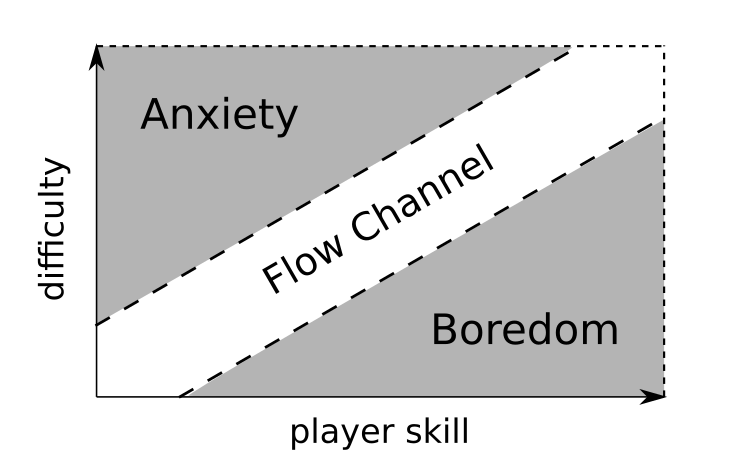
\includegraphics[width=26em]{figures/fig-flow-channel.png}
    \end{center}
    \legend{Source: Diagram assembled by the authors based on the concepts defined by \cite{BOOK_Flow}.}
    \label{fig:flow-channel}
\end{figure}

The balance between challenge and skill strongly contributes to the optimal experience of a player, and is referred to as a defining factor on the quality of a game \cite{ARTICLE_FearOfFailure}. We argue that we can balance the level of challenge through AGT. By acquiring information on the profile and preferences of a player, we can either ramp up the difficulty or encourage the learning process. Therefore, we understand that the usage of AGT can directly contribute to a positive experience.

\subsection{Learning Curve}
\label{sec:learning-curve}

Another interesting concept in games is the \emph{learning curve} \cite{article_learningcurve}. The learning curve depicts how easy it is to become used to the game's mechanics and systems. Game Developers often consider the learning curve as a key reference when performing level design. The first few levels of a game should enable the player to learn each mechanic in an isolated and controlled environment, whereas the last levels of a game should be designed considering that the player has knowledge about all the mechanics proposed by the game designer, and thus should present challenges that require mastery of each mechanic to surpass. Figure \ref{fig:difficulty-curves} depicts multiple possibilities for difficulty curves as a function of player progress in a game.

\begin{figure}
    \caption{Examples of the distribution of difficulty in games as a function of player progress.}
    \begin{center}
        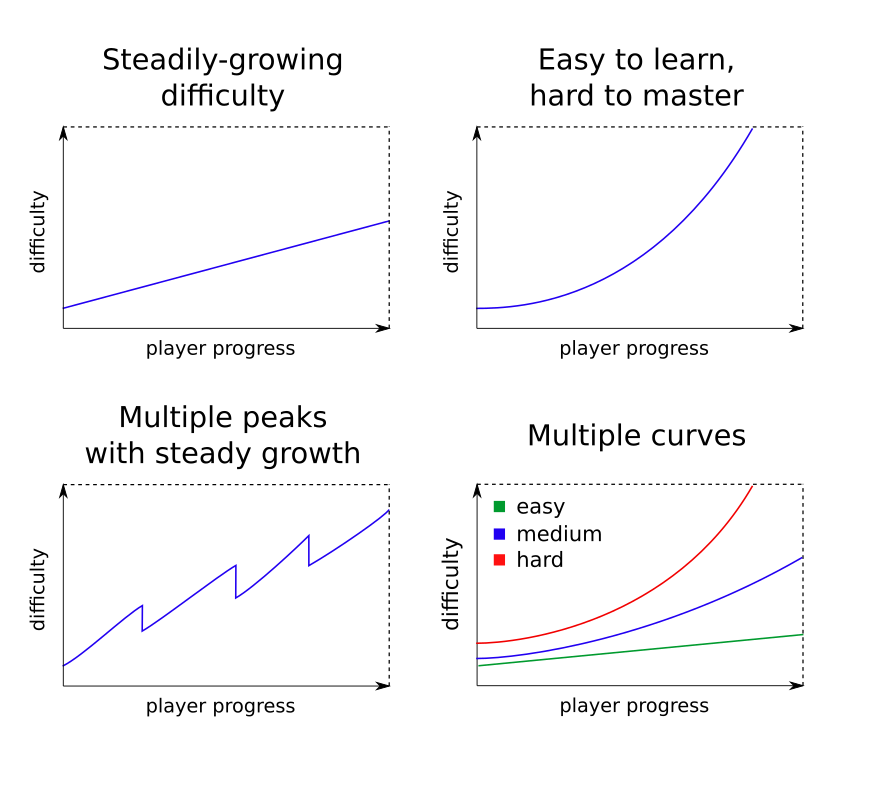
\includegraphics[width=26em]{figures/fig-difficulty-curves.png}
    \end{center}
    \legend{Source: Diagram assembled by the authors.}
    \label{fig:difficulty-curves}
\end{figure}

Perhaps the most notable example in teaching game mechanics through a concise learning curve is seen the famous game \emph{Super Mario Bros} \footnote{Super Mario Bros (Nintendo, 1985). Video Game. Nintendo Entertainment System.} in World 1-1, as addressed in \cite{video_extracreditsmario11}. In the first thirty seconds of gameplay, the player is able to learn that they must progress going to the right, that enemies must be avoided or eliminated by jumping in their heads and that special blocks hide valuable rewards such as additional lives. All the mechanics are taught without a single line of text or on-screen dialog box. Instead, the game teaches them by simply using the player's curiosity with an ingenious placement of game entities.

Some genres of games with consolidated and well-known mechanics share multiple similarities. The mechanics in such genres are proven to be one of the core constituents in their type of gameplay, and are expected by any non-novice player. One example would be the FPS (First Person Shooter) mechanics of \emph{Call of Duty: Modern Warfare}\footnote{Call of Duty: Modern Warfare (Infinity Ward, 2007). Computer Game. Microsoft Windows.}. The running, sprinting, strafing, vaulting, proning and iron-sighting mechanics were so exceptionally well done that they still remain in the most recent title of the series, \emph{Call of Duty: Black Ops 4}\footnote{Call of Duty: Black Ops 4 (Treyarch, 2018). Computer Game. Microsoft Windows.}. Other entries in the FPS genre such as \emph{Battlefield}\footnote{Battlefield 5 (DICE, 2018). Computer Game. Microsoft Windows.} also employ the same set of mechanics, which has since then become almost a requirement for the non-tactical Arcade Shooter style.

Arguably, games with the mechanics of a consolidated genre have a faster initial learning curve to any player that has played a similar game before. These games take advantage of that, and throw the player straight into the action. Within the first few minutes of playing a \emph{Call of Duty} game, the player will have faced and beaten an impressive amount of enemies. They will also confirm their proficiency by choosing exactly the difficulty level that appeals to their skill. Therefore, the veteran player of such a genre knows what to expect of the game and its standard difficulty level. They tailor their game experience to the optimal experience in the act of leisure.

We argue that Adaptive Game Technologies can also have an impact on the learning curve issue. Understanding the profile of a player before gameplay takes place can be a key factor on the decision to ramp up the initial challenge of a game, and remove or alter initial sections which only serve the purpose of teaching basic mechanics.

Thus, the learning curve should not be static, but customized to the needs of each player. If the player has already mastered the base concepts of a game, they should be encouraged to using their knowledge to the fullest. Tailoring the learning experience to each player could balance the challenges faced by the player to a more appropriate, which could possibly increase the sense of enjoyment and immersion as seen in \autoref{sec:challenge-flow}.

% =======================================================
% PLAYER MODELING
% =======================================================

\subsection{Player Modelling}

The concept of adaptivity in games relates to how a game is able to adapt its content based on the \emph{profile} and \emph{preferences} of a player, which constitute \emph{player models} obtained from a multitude of \emph{Player Modelling} techniques. Player Modelling allows the creation, collection and processing of \emph{player models}, real-time collected data sets that can be classified into reality-based player types \cite{ARTICLE_DynamicPlayerModelling}. Knowledge about player types allows dynamic adjustment in the sense of content customization, where a game designer might dynamically assign what should be presented to each type of player.

In a DDA system, \emph{Player Models} refer to collections of data gathered to be used as a metric for adjustment policies \cite{PHD_DynamicDifficultyAdjustment}. Player Model data might be gathered during a play session as a trace of the player's actions and events in a game, or as static data collected from surveys or through the use of a gaming platform such as \emph{Steam}.

One possible implementation of a \emph{Player Model} consists of defining a collection of numerical attributes that describe the playing style of an individual player, as seen in \cite{BOOK_PlayerModeling}. Each attribute defines an aspect of the player's behavior, which is generally associated with their strategy or mechanical skill. A typical example of Player Model in a Shooter game can be seen in Listing \ref{lst:PlayerModellingExample}.

\begin{lstlisting}[caption={Example of a Player Model for a shooter game.},label={lst:PlayerModellingExample}]
class PlayerModel {
  public:
    enum Attribute {
      bCanStrafe,
      bCanFlick,
      bDoesStationaryShooting,
      fPrecision,
      fEncounterDuration,
      fKillsPerRound,
      fDamagePerRound,
      fDistancePerRound
    }
    void Initialize();
    void UpdateAttribute(Attribute att, float newValue);
    float GetAttribute(Attribute att);
    private:
      vector<float> attributeValues;
};
\end{lstlisting}

The values for each attribute are unknown to the game preceding a session. Therefore, it is necessary to sample and adjust the values during gameplay. Each time a sample is collected, the Player Model should reflect a player's behavior with increasing precision. In the implementation proposed by \citet{BOOK_PlayerModeling}, the attribute update function uses the \emph{Least Mean Squares} (LMS) training rule, commonly used in machine learning:

\begin{lstlisting}[caption={Implementation of attribute update using least mean squares.},label={lst:AttributeUpdate}]
float UpdateAttribute(Attribute att, float value) {
    float currvalue = attributeValues[att]; N
    float delta = value - currvalue;
    float weightedDelta = LEARNING_RATE * delta;
    attributeValues[att] += weightedDelta;
}
\end{lstlisting}

Attributes in this implementation consist of values between 0 and 1, indicating the probability of a player performing an action. In Listing \ref{lst:PlayerModellingExample}, this can be seen in the definitions of Boolean attributes (prefix 'b'). However, it is also possible to use the same approach to approximate statistical values, such as the damage a player inflicts per round. The value for each attribute represents the game's current best guess. Each sample collected contributes to the estimate weighted by LEARNING\_RATE. Therefore, for lower LEARNING\_RATE values more samples are required to sufficiently approximate an attribute. In most cases, values between 0.1 and 0.3 are used \cite{BOOK_PlayerModeling}.

The concept of player models is used as a basis for dynamic adjustments in the framework described in \cite{ARTICLE_DynamicPlayerModelling}. The authors describe a methodology for the conception of player models that considers the existence of \emph{concept drift}, which is the possibility of players adapting or changing behaviors and play styles according to their evolution or progress in a game. The framework relies on two sources of data related to players: information of player preferences inputted by a player prior to application use and tracking player performance in-game. Figure \ref{fig:dynamic-player-model} exemplifies the dynamic player model framework.

\begin{figure}[!ht]
    \caption{A representation of the dynamic player modelling framework discussed in \cite{ARTICLE_DynamicPlayerModelling}.}
    \begin{center}
        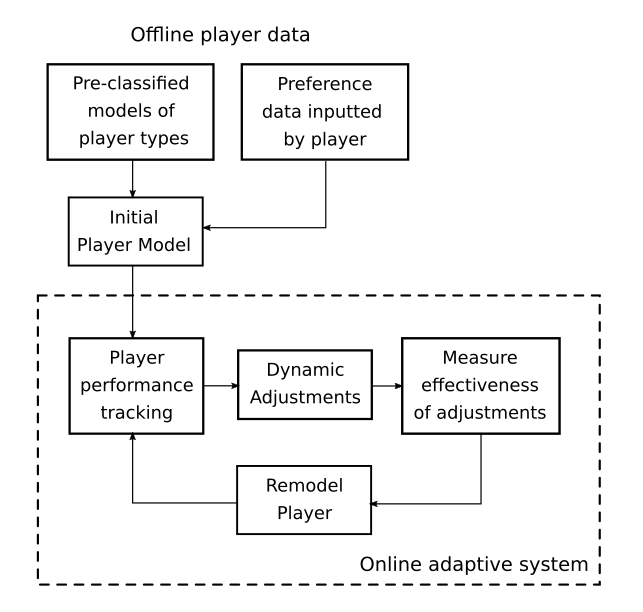
\includegraphics[width=26em]{figures/fig-dynamic-player-model.png}
    \end{center}
    \legend{Source: Diagram assembled by the authors based on visual representations in \cite{ARTICLE_DynamicPlayerModelling}.}
    \label{fig:dynamic-player-model}
\end{figure}

The discussion in \cite{ARTICLE_DynamicPlayerModelling} emphasizes the necessity of remodelling player types after measuring the effectiveness of adaptation. This means that a DDA system should be able to gather some type of player feedback regarding the effectiveness of the dynamic adjustments that were performed during play, and recreate the player profile based on this feedback. Some methods for gathering such feedback include inferring the player's affective state, such as with physiological sensors or from a camera or an analysis of statistical data retrieved from in-game attributes, such as player performance or their action history.

\subsection{Dynamic Adjustments}

Mechanisms for adaptive adjustments should describe what elements of the game are going to be monitored, and what variables should be adjusted accordingly. Therefore, the functionality of a DDA system can be summarized as a relation between observation and adjustment. Since video games are so diverse in design and functionality, the mapping between observation parameters and adjustment variables has yet not been efficiently described as an universal and generic approach \cite{PHD_DynamicDifficultyAdjustment}. Rather, the game developer should decide what variables should be observed and adjusted in a per-game basis.

\section{Adaptive Systems In Research}
% * ======================================================================
% * ======================================================================
% *  ADAPTIVE SYSTEMS IN RESEARCH
% * ======================================================================
% * ======================================================================

Previous academic work regarding adaptive system implementations include novelty approaches with innovative metrics and adjustment policies that affect a variety of systems or mechanics. In this section, we use the literary review in \cite{article_ddareview} as a reference to classify DDA algorithms implemented in previous academic work, as well as to select analyze the most relevant implementations for each of the proposed methods.

\subsection{Probability-based DDA Systems}
\label{sec:statistical-adjustments}
% * =======================================================
% *  PROBABILISTIC DDA
% * =======================================================

% * Footnotes
% * ================

\sepfootnotecontent{fn:half-life-1}{Half-Life (Valve Software, 1998). Computer Game. Microsoft Windows.}

\sepfootnotecontent{fn:healing-items}{Healing items in games are consumable resources that restore a percentage of the maximum health points of a player. An example for this are the health stations in the Half-Life franchise, where the player heals up to 80\% of their maximum health points upon interaction, but the resource is permanently depleted after use.}

% * Overview of the Hamlet system
% * ================

One of the pioneer implementations of adaptive systems in research is the probabilistic model approach in the Hamlet system, as seen in \cite{article_casefordynamicdifficulty}. Hamlet is a probability-based predictive system that is able to perform reactive and proactive adjustments to the distribution of items throughout levels of customized Half-Life \sepfootnote{fn:half-life-1} map. The general methodology proposed by the system involves defining a finite set of possible gameplay states based on contextual information of player status, and performing adjustments based on policies defined by such metrics. The objective of the system is to avoid "game state loops", where a player would perform the same set of actions repeatedly when failing through a specific segment of the game.

\subsubsection{Methodology and Results} 
% * How the Hamlet system works
% * ================

% Hamlet establishes probabilistic distribution of damage done to player
% Probability of death can be estimated when relating damage with enemy types
% Probability of death is a composite metric based on player performance
First, the system establishes the probabilistic distribution of damage done to the player by registering changes to the value of player health over time, as well as the source factor for each change. By relating change occurrences in the health attribute with each of the enemy classes, the probability of the player dying during an encounter can be estimated, given that the enemy types that will be presented in a future encounter are known. The probability of player death is the metric used as input for adjustment policies in the Hamlet system, and is calculated from statistical data regarding \emph{player performance} during previous combat encounters.

% If probability of death > 40%, system distributes healing items
% This is an example of proactive adjustment, before game events
If the probability of death for an encounter is above 40\%, the system intervenes by distributing \emph{healing items}\sepfootnote{fn:healing-items} throughout the level before an encounter takes place. The distribution of healing items before combat encounters based on probabilistic metrics can be classified as a \emph{proactive adjustment}, as it occurs before an undesired in-game event such as player death.

% Reactive Adjustments: maximum enemy HP, enemy accuracy
% Objective is to decrease of health lost, reducing repeated deaths
% Target value for mean health is 60%, with 15% standard deviation
The Hamlet System also implements \emph{reactive adjustment} policies which occur during combat encounters, such as adjusting the maximum hit points for an enemy type or modifying the accuracy of shots fired by enemies. The objective of these adjustments is to decrease the amount of health lost by players during combat encounters, consequently reducing repeated death occurrences.The target value for the mean health percentage is 60\%, with a standard deviation of 15\% at most segments of the game.

% * Results of the Hamlet System
% * ================

% Results showed that most players were unable to recognize adjustments
% Some players suggested adjustments that did not exist
% Several players suggested that the system did not perform any adjustments
Results of experimentation using the Hamlet system showed that most players were unable to recognize when the system was performing adjustments, or characteristics of the game were modified when adjustments were performed. Some players suggested that the system performed adjustments that were not there, and several players suggested that the system did not perform any adjustments based on their skill level.

% Proactive adjustments are harder to measure in comparison to reactive
% Variations in skill level might not be considered
% Requires predefined constraints to provide proper level of challenge
The authors argue that the cause for incorrect perceptions of users regarding the adaptive system is related to the fact that the effects of proactive adjustments are harder to measure in comparison to \emph{reactive adjustments}. Variations in the performance of a player caused by an increase of the skill level might not be considered as an input to the adjustment policies. Therefore, this type of adjustment should be performed with predefined constraints determined by the game designer in order to properly reflect the intended level of challenge.

% Slight correlation between adjustments and enjoyment for expert players
% Player performance is increased without players understanding why
% However, novice players do not perceive changes
During the post evaluation interviews, the authors noticed a slight correlation between the adjustment policies and player enjoyment when considering players with an expert skill level, where adjustment policies positively affected player performance without the players being able to identify which aspects of the game were modified. However, novice players with a lower level of skill did not report any perceivable change.

% Adjustments can improve performance without affecting sense of agency
% When in harmony with game design, adjustments can be imperceptible
The study concluded that adjustment algorithms can improve the performance of a player while retaining the player's sense of agency and control. When performed with accordance to the game's core design adjustments can be nearly imperceptible, slightly increasing the sense of enjoyment of a player without diverging from the proposed experience.

\subsubsection{Analysis of Positive and Negative Aspects}
% * Positive Aspects of Hamlet System
% * ================

% Can be integrated in the game development process during or after development to modify already existing difficulty parameters, as evidenced by the fact that the approach was applied by modifying the original Half-Life Game
One of the positive aspects of probabilistic approaches that use player performance metrics as input is regarding to their feasibility of implementation in already existing games, as evidenced by the fact that the methodology implemented in \cite{article_casefordynamicdifficulty} was applied by modifying the original Half-Life game. Therefore, the necessity for such adjustment algorithms can be considered and evaluated during or after the process of the original design iterations, and can be discarded if considered unnecessary.

% Predictive solution which can reduce frustration before undesired in-game events occur
% Combined with reactive adjustments can provide immediate real time solution to discrepancy between player skill and proposed challenge level
Another positive characteristic relates to the nature of predictive adjustments, where undesired in-game events can be prevented before a first occurrence, which might have a positive result in reducing player frustration. Combined with reactive adjustments, this methodology can provide immediate and real-time solutions to the discrepancy between player skill and the proposed challenge level of a segment in the game before and during first traversal by the player.

% * Negative Aspects of Hamlet System
% * ================

% While it can alleviate difficulty curve, might be hard to adjust
% Becomes difficult for game designer to understand results
%    - Adjustments are performed before or during first traversal by the player
However, we argue that while probabilistic systems this might be  interesting as a supportive DDA implementations that can alleviate the difficulty curve of a challenging game, they might prove to be hard to adjust and customize from the perspective of game designers. It becomes difficult for a game designer to predict or understand the results of the integration and modifications of such an approach when the adjustments are performed before or during the first traversal of the player through game segments.

% Probability estimations don't consider player improvements
% System modifies encounters before player has a chance to improve
% May be good to reduce frustration for novices, but slows learning process
Additionally, probability estimations are generally ignorant to immediate variations in player performance caused by a change of strategy or even an increase in the quality of mechanical execution performed by the player. It can be argued that the system attempts to modify the outcomes of in-game events before the player has a chance to fail, and consequently attempt to improve their strategies and execution to succeed in a combat encounter. Therefore, while this approach may reduce frustration for cases where a player is unable to handle the level of challenge, it may also hinder or slow player progress in regards to their skill.

% \subsubsection{Alternative Implementations} 
% TODO * Examples of Other Probability-based systems in Research
% * ================

\subsection{Affect-based DDA Systems}
% * =======================================================
% *  AFFECT-BASED DDA
% * =======================================================

% * Footnotes
% * ================

\sepfootnotecontent{fn:cutscene}{A \emph{cutscene} is a special in-game event where the player is unable to input control into the game, and audiovisual feedback is a result of an automatic, predefined sequence of events determined by the game developers. Cutscenes can be seen as parts of a game that are similar to a movie, where the game is not interactive and instead focuses on telling a part of the story.}

% * Overview of the Affect-Based systems
% * ================

% Most DDA methods use profile or performance
% Work in affectivedda uses affective state
% In affectivedda, body signals are metrics to adjustment policies
% Ultimately anxiety level increases or decreases difficulty
Most implementations of DDA systems analyzed in the scope of this work use metrics that represent player profile or performance as input to the adjustment policies. However, a different approach can be taken when using player emotional state as both an input and a feedback mechanism when modifying difficulty. This is the theme of the work presented in \cite{article_affectivedda}, where physiological signals were tracked to infer the anxiety level of players, and then used as a metric to perform difficulty adjustments which cause a reduced or increased feeling of tension throughout the game.

\subsubsection{Methodology and Results}
% * How affect-based systems work
% * ================

% Unused
% ========================================
% Electrodermal and cardiovascular activity are related to anxiety
% Increase in skin conductance can be caused by anxiety
% Decrease of parasympathetic activity may also suggest anxiety
% The research performed in \citet{article_affectivedda} cites previous literature to understand which physiological signals can be used to infer the anxiety levels of a user. It is observed that \emph{electrodermal} and \emph{cardiovascular} activities have a relation to anxiety levels, as well as increases in skin conductance levels. A decrease of parasympathetic activity and increase in sympathetic activity in the heart also presented relation to anxiety.

% Unused
% ========================================
% Blood pulse volume measured at fingers were also shown to be subject to stress manipulation, and presents a correlation with self-reported anxiety \cite{article_affectivedda}. Measures of EMG (Electromyography) activity of specific muscles (such as Corrugator Supercilii) were also shown to be strong indicators of anxiety.

% Adaptive syste, uses cardiovascular, electrodermal and EMG activity as input
% RT technique classifies physiological signals into affective states of anxiety levels
The adaptive system implementation presented in \cite{article_affectivedda} uses features of cardiovascular activity (inter-beat interval, relative pulse volume, pulse transit time and heart sound), electrodermal activity (tonic and phasic response to skin conductance) and EMG activity (from Corrugator Supercilii, Zygomaticus and upper Trapezius muscles) as input data to a Regression Tree (RT) technique, which classifies the physiological signals into affective states that categorize anxiety levels.

% Object of study was a pong-based games
% Two variations: adjustments based on performance and based on affective state
A \emph{Pong}-based game was implemented for the study, with two variations in difficulty adjustment algorithm: one where the difficulty would be adapted based on player performance (a relationship between points scored against or in favor of the player), and another where the anxiety level of the player is used as input to alter difficulty.

% Three difficulty levels
% Performance: Excellent, Poor performance causes difficulty changes
% Anxiety: High and Low anxiety causes difficulty changes
Three difficulty levels were implemented in total, which would be assigned depending on performance or anxiety levels: if the player's performance is classified as "Excellent", the player would progress into the next difficulty level. If the performance is classified as "Poor", the difficulty level would be decreased. The affect-based variant utilizes an analogue solution, where the difficulty is increased if the anxiety level is classified as "Low", and the difficulty is decreased if the anxiety level is classified as "High". Figure \ref{fig:affective-adaptation} displays state-flow diagrams representing the difficulty levels and their transition conditions.

% * Figure: Performance-based and anxiety based adaptation
% * ================
\begin{figure}[!h]
    \caption{A state-flow diagram representation of the performance-based and anxiety-based adaptation variants in \cite{article_affectivedda}.}
    \begin{center}
        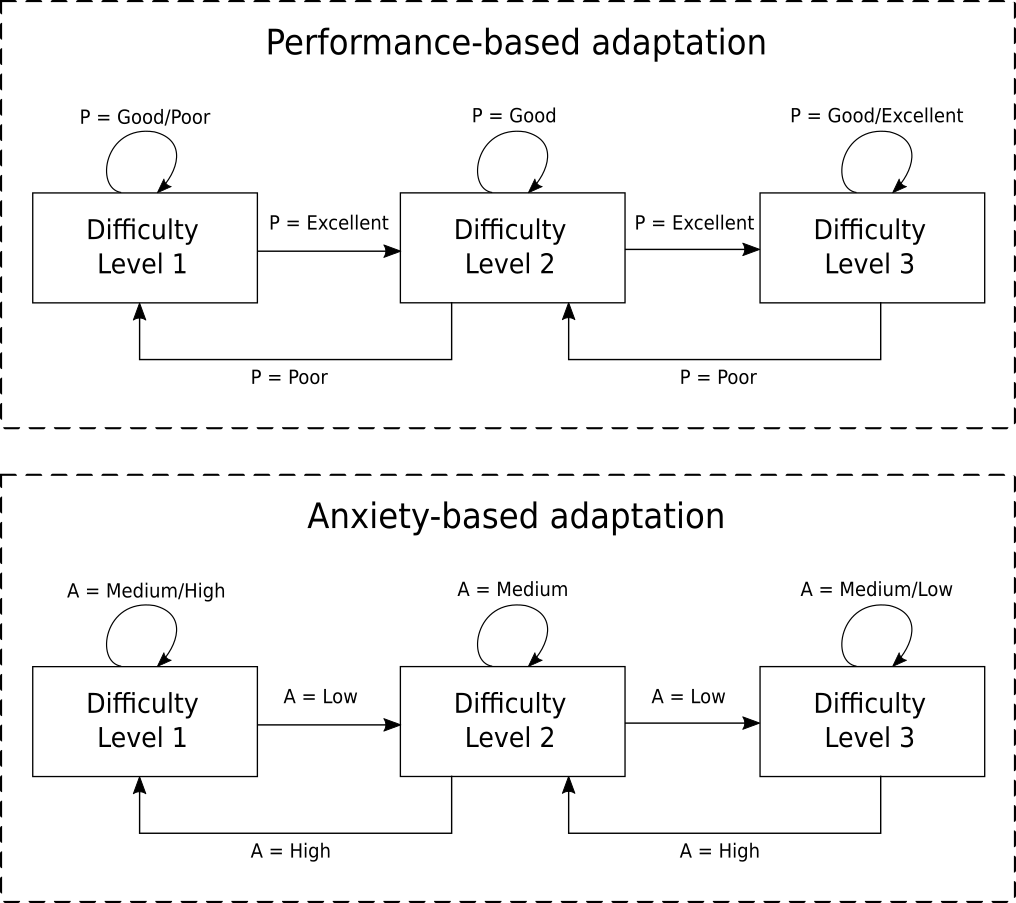
\includegraphics[width=26em]{figures/fig-affective-adaptation.png}
    \end{center}
    \legend{Source: Diagram assembled by the authors based on visual representations in \cite{article_affectivedda}.}
    \label{fig:affective-adaptation}
\end{figure}

% * Results of Affect-based System
% * ================

% Regarding performance, most players showed improvement in affective over performance metrics
% Could be justified as Pong becomes more difficult over time, increasing tension
Regarding the impact of affect-based adaptation on player performance, results of the experiment showed that the performance of most players showed significant improvement in the adjustment method which used affect-based metrics as an input, in comparison to the method which used performance metrics.  This could be justified by the fact that in a Pong-based game, the game becomes progressively more difficult over time with an increase of the speed of the ball, causing feelings of tension as either the player or an AI-controlled opponent are closer to scoring a point.

% Increase of tension causes variation in anxiety levels, changing difficulty in real-time
% Change of difficulty in this case is a proactive adjustment
% Goes in contrast with performance-based reactive adjustments
The increase of tension causes variations in physiological signals that classify as increases in the anxiety level, and thus the difficulty adjustment might be performed before the player or an AI agent is able to score. This could be argued to classify as another example of \emph{proactive adjustment}, which goes in contrast to performance-based adjustments which are \emph{reactive adjustments} by definition as the only metric used as input are outcomes of in-game events. 

% Players perceived affect-based version to be more challenging
%   - Could also be justified by real-time proactive adjustments
%   - Players have little time to relax before difficulty increases again
% Players reported that the affect-based version was more satisfying
%   - What is the justification for this?
Players also perceived that the DDA implementation which used affect-based metrics for adjustments was more challenging than the performance-based DDA version. This could also be justified by the nature of the real-time adjustments that were implemented. Instead of being based on the outcomes of in-game events (which in this case involves player and AI opponent scores), the difficulty is directly mapped to the level of anxiety of the player.

When the player is able to score and attain a lead over the AI opponent, they might feel a sense of relaxation which decreases the anxiety level. Consequently, the system detects the change in the affective state and increases the difficulty accordingly. However, the most crucial difference to the performance-based implementation could be attributed to the fact that the difference in anxiety level when the player achieves a small numeric lead might be much more significant than estimation of performance from the score difference in the performance-based solution, when considering the same scores for player and AI. This could cause the match to become much more competitive in the affect-based version, as the AI opponent would present a much higher difficulty even when the player attains small leads.

Additionally, players reported that the affective version was more satisfying. In the same sense that a real-time anxiety based metric can adjust the difficulty based on an increase of the tension level, it could also be able to identify moments where players feel more relaxed, an affective state which can cause boredom if maintained over a prolonged duration, as discussed in the earlier sections of this chapter. Combining this with the earlier discussed fact that a match can become much more competitive due to the discrepancy between anxiety levels and performance statistics, the player might feel a higher sense of reward when achieving victory over an opponent which is perceived as more challenging.

\subsubsection{Analysis of Positive and Negative Aspects}
% * Positive Aspects of Affect-based systems
% * ================

Considering the results of the affect-based DDA implementation in comparison to the traditional approach of performance-based metrics, we can begin to identify some of the advantages of using real-time tracking of physiological signals and affective state classification in regards to the restrictions that are inherent to event-based capturing of gameplay data.

 % Affective-based metrics might not require the same amount of data or time to perform adjustments as performance-based metrics, as they are not bound to the rules of a game
We can begin by arguing that affect-based metrics might not require the same amount of data or time to be used as input by adjustment policies in comparison to performance-based metrics, as they are not bound to the rules or domain of a specific game. The gathering of physiological signals and classification of affective state is agnostic to the object of study in itself, as it simply involves the external use of sensors and a classification methodology to output an estimate of the player affective state.

The use of the information on such affective state must then be considered by game designers to determine which systems it might affect. In the work described in \cite{article_affectivedda}, the affective state was used as input to adjust the difficulty of an AI opponent, but affective metrics are not restricted to being employed on difficulty adjustment systems.

 % In contrast to other methods, the input for metrics is directly mapped to the proposed feedback
 % As discussed earlier, affective state is one of the main constituents of player experience
 In contrast to traditional DDA implementations which involve metrics that are limited to the events of a game, the input in affect-based DDA approaches can be directly mapped to the desired changes in the affective state of a player. As discussed earlier in this chapter, the affective state of a player is one of the main constituents of player experience, which makes this approach especially interesting considering the objective of maintaining a challenging difficulty level to the player but at the same time avoiding frustrating situations.  

 % Affective-based adjustments are performed in real time
 % Adjustments might occur in anticipation of in-game events, which is a proactive approach
 The implementation in \cite{article_affectivedda} involved real-time classification and validation of adjustment policies, which meant that the adjustments might occur in anticipation of undesired in-game events that can cause frustration. Therefore, it can be argued that this implementation defines a proactive adjustment methodology which might provide an immediate or preventive solution to possible frustrating events, when being compared to traditional performance-based adjustments.

% * Negative Aspects of Affect-based systems
% * ================

% Implementation is not feasible in commercial games in the present
% Current hardware does not track relevant physiological signals
While the research on affect-based DDA showed mostly positive results in comparison to performance-based metrics, it could be argued that employing this type of solution in a commercial video game is not feasible, as current hardware used in modern video-game consoles does not include or support sensors capable of tracking significant physiological signals that can be used to determine affective state.

% If hardware in home consoles evolves to be able to track physiological signals, there is still the problem of appropriately integrating affect-based adjustments in the game development process
% During playtesting, affective state has to be monitored and compared to the experience proposed by game designers, which creates restrictions and possible slowdowns in iterative development
If improvements in hardware used in video-game consoles evolve in the direction of including sensors that are able to track relevant physiological signals that can determine affective state, there is still the problem of appropriately integrating affect-based adjustments in the game development process. During play-testing sessions, the affective state has to be monitored and compared to the values that are expected by game designers, which creates restrictions and possible slowdowns in the iterative process of game design balancing and refinement.

% Methodology was applied to a simplistic game implementation
% Experiment should be performed in a modern game which can promote more affective states
Furthermore, the game implementation used for the experiment is a simplistic game with limited audiovisual feedback. As discussed earlier, audiovisual feedback is one of the factors that can contribute to player experience, and consequently to the affective state of the player. Therefore, research with affect-based DDA systems should be continued as to perform similar experiments in modern games with high audiovisual fidelity. Modern games are often able to evoke a multitude affective reactions by immersing the player with more recent technology, features or systems such as \emph{cutscenes} \sepfootnote{fn:cutscene} or visual and audio effects, and the integration of affect-based adjustments in modern games can prove to be a challenging task, as it might not involve simple adjustments in difficulty parameters.

% \subsubsection{Alternative Implementations}
% TODO * Other Implementations of Affect-based systems in research
% * ================

\subsection{Learning-based DDA Systems}
% * =======================================================
% *  LEARNING-BASED DDA
% * =======================================================

% * Footnotes
% * ================

\sepfootnotecontent{fn:waypoints}{A \emph{waypoint} is a special position in a game world where an in-game event is toggled when the player is within interaction range. Waypoints are commonly used in games when the player has to take a specific path to a goal, with the game assigning several intermediary positions the player has to pass through to validate that the correct path was taken. In the context used for the implementation presented in \cite{article_adaptivebehaviorai}, waypoints are simply game world positions the cars must reach to score points. Each time one of these positions is occupied by a car, the waypoint is destroyed and a new random position is assigned elsewhere in the game world as the next waypoint.}

% * Overview of Learning-Based DDA
% * ================

Another approach to adaptive difficulty involves the adaptation of AI (Artificial Intelligence) agent behaviors through reinforcement learning. 

\subsubsection{Methodology and Results}
% * How Learning-Based DDA works
% * ================

% Modifies behavior of AI agents in car race game
% Objective in game is to pass max. number of waypoints in limited time
% Multiple waypoints at screen in any given time
% Waypoints disappear when passed through
The implementation of learning-based DDA in \cite{article_adaptivebehaviorai} adjusts the behavior of AI agents in a simple car simulation race game, where each player has the objective of passing through the maximum number of \emph{waypoints}\sepfootnote{fn:waypoints} in a given amount of time. Multiple waypoints are displayed on the screen at all times, and a waypoint disappears when any of the players approaches close enough for interaction range.

% Two types of behavior AI Components
% First layer is driving functionality, motor controls
% Second layer is tactical behavior, outplay opponent
The AI agents implemented define two types of behavioral AI components. The first type is defined by components associated with driving functionality, with the objective of improving driving performance of the controller. The second type is associated with behavioral components that affect the tactical decisions of an AI agent, and have the purpose of performing actions that outplay their opponent.

% Driving components focus on car controlling
% Tactical behavior components decide which waypoint to head to
% Driving components can be seen as mechanical input
% Tactical behavior components influence high-level decision making
Driving behavior components ignore the existence of the opponent, instead focusing on simply performing actions required to drive the car. Tactical behavior components help the AI controller decide which waypoint to head to, or if the controller should not head to a waypoint at all. In a more general perspective, the Driving Behavior components can be seen as the mechanical input of AI agents in the game, whereas the Tactical Behavior components influence the high-level decision making process of the AI agent. 

% 7 components implemented, 3 driving and 4 tactical
% Each component does not override the others
% It is possible to have all 7 components activated at the same time
In total, 7 components were implemented, with 3 being driving behavior components and 4 being tactical behavior components. Each component is restricted to executing a set of actions that does not conflict or override actions of other components, which means it is possible to define an AI agent that uses all the behavior components implemented for the application.

% Two evolutionary computation algorithms: AUC and ADC
% Advantage of such training methods is being performed online
To evaluate the performance of each component, two evolutionary computation algorithms are implemented: the adaptive uni-chromosome controller (AUC) and the adaptive duo-chromosome controller (ADC). The advantage of using such algorithms is that the training and adaptation process can be performed online and in real time, over the course of a game session.

% Each chromosome stores seven real numbers
% Each number defines probability of activating a component
% Two metrics for input:
%   - Minimization of the winning percentage difference
%   - Minimization of the mean score difference
Each chromosome in the AUC and ADC algorithms stores seven real numbers representing the probability of activating a behavioral component whenever a waypoint is passed. Two metrics are used as an input for the adaptation algorithm: first, a minimization of the winning percentage difference (|W - L|, where W represents the wins and L represents the losses) and second, a minimization of the mean score difference (|s1-s2| where s1 and s2 represent the scores of player 1 and player 2).

% Evaluate efficiency of adjustments by enabling all components
% Against 5 static AI components with random traits
To evaluate the efficiency of the adaptation algorithms, the authors first compared the strongest AI agent that the adaptive system would possibly generate (which would be defined by enabling all behavioral components simultaneously and permanently) against five static AI controllers based on various traits that would simulate various styles of play, such as heuristic controllers, reverse-enabled controllers, predictive fast controllers, and neural network controllers.

Sets of \emph{n = 5000} games were played for each opponent in each step of the experiment. Through the first step of the experiment, the authors validated that a fully-enabled adaptive AI controller (having all the behavioral components activated at all times) was a competent opponent with positive median score differences against all static AI controllers.

In sequence, the authors conceptualized AI agents where behavioral components were activated randomly whenever a waypoint was crossed. The objective of this approach was to demonstrate that some sort of adjustment algorithm that considers opponent strategies is necessary for different types of opponents, as randomly assigned behaviors are not able to present consistent results against a fixed strategy. Results showed that the random behavior selection algorithm had negative median score differences against all five static controllers.

% * Results of Learning-Based DDA
% * ================

In the third step of the experiment, the authors evaluated the use of the AUC algorithm. The expected behavior set encoded by a chromosome as a result of the algorithm should represent a "winning" strategy. Effects of varying \emph{Learning Rate} and \emph{Mutation Rate} were documented for the experiment, showing that the general trend of increasing learning rate is a gentle increase in the mean score difference, since a large learning rate quickly saturates chromosome values. Higher mutation rates tend to produce larger differences in mean score and winning percentage by producing large fluctuations in chromosome values. In general, high mutation rates led to poorer results.

In the final step of the experiment, the use of the ADC algorithm was evaluated, with the same idea of varying the Learning and Mutation Rates. For the ADC algorithm, no trends were perceived in association with varying Learning rates. This would likely have been caused by the reduction of the frequency of update opportunities for each chromosome. In the ADC algorithm, only one of two chromosomes is updated each time a waypoint is passed. This means that on average each chromosome is updated half as frequently as chromosomes in the AUC variant. As for the Mutation rate, the results of the ADC controller improved greatly as mutation was introduced, possibly because the mutation operation offered more opportunities for the chromosome values to adapt.

As a conclusion to the experiment, the authors expressed that while the AUC algorithm had lower memory footprint, the ADC algorithm was able to better minimize the number of drawn games, which would possibly reduce player frustration. It was also noted that both the AUC and ADC algorithms were able to generate specific patterns of behavioral component distribution for each of the static controller stereotypes, meaning that the Reinforcement Learning technique would be able to adapt to different styles of play. The general intent of both algorithms was not to maximize the number of wins, but to maintain a fair and close challenge to the opponent by minimizing the score difference as well as the difference between number of wins and losses.

\subsubsection{Analysis of Positive and Negative Aspects}
% * Positive Aspects of Learning-Based DDA
% * ================

% Novelty approach: unsupervised online learning
% Lessens responsibility of game designer tailoring adjustments
The work presented in \cite{article_adaptivebehaviorai} introduces the novelty approach of online learning without predefined data sets to the scenario of DDA solutions. It could be argued that the adjustment policies are also part of the reinforcement learning approach, since the decision of a behavioral component being activated or not relies on the algorithm being applied. This is an especially interesting solution since it lessens the responsibility of a game designer tailoring the boundaries of the adjustment system in advance of play.

% Could be applied to create AI agents that replicate player behavior in online games, where massive data sets can be gathered from large audiences
One interesting application to methods which implement online learning without predefined data sets would be highly popular online multi-player games, where data from thousands of matches can be gathered each day, which provides a massive amount of input for training algorithms. This can be used to speed up the process of training AI agents to perform the most appropriate actions given a situation, which in turn will provide a more competitive challenge to players.

% * Negative Aspects of Learning-Based DDA
% * ================

% Experiment was not performed using real players
% Long time to train agents means long time for opponents provide a fair challenge, which can cause frustration to players
However, we argue that this experiment has yet to be applied in the context of real players using an implementation that would better replicate a commercial video game product. Learning algorithms might require a long time to train agents to the point of providing a fair challenge to players, which might cause frustration and negative bias in player perception regarding the AI design.

% Simplistic game implementation, modern games present many more components regarding AI, which would mean much more time to train
Additionally, the work implemented in \cite{article_adaptivebehaviorai} uses a simplistic game implementation as an object of study, where the objectives and available actions are restricted to few options which simplifies the implementation of behavioral components and in consequence reduces the amount of data, processing and time to train agents.

In modern video games which present sophisticated AI solutions, the amount of information regarding game state and actions that a player or AI agent can perform can be dramatically higher in comparison, which means that the amount of behavioral components would be much higher, and consequently result in an exponential increase in the amount of data, processing power and training time -- to the point of becoming unfeasible to integrate in a project, as modern games commonly allocate most processing power of hardware to the execution of its rendering and gameplay systems.

% Unsupervised learning might cause game designer to lose control over the balancing of AI opponents
% Adjustments are based on keeping the challenge at a fair and competitive level, but game designers might purposefully want to design a section of the game with a significant increase in challenge level to increase tension or cause specific affective reactions
Another problem surfaces when considering balancing and adjustments of AI opponents by game designers under the iterative nature of the game development process. In the specific case of the implementation in \cite{article_adaptivebehaviorai}, as in-game parameters such car speed and handling are modified, the data which defined the training sets for AI agents might have to be discarded, as actions that would previously define a winning strategy could become obsolete by the changes in car physics. 

Therefore, simple adjustments to the balancing of a game might cause the learning-based AI to have to be re-trained. Since the balancing of a game is also dependant on the difficulty of AI opponents, which in this case is defined by data accumulated from multiple matches, integrating such a process in iterative game development becomes unfeasible, as small changes to the game would cause all AI opponents to become unbalanced.

% \subsubsection{Alternative Implementations}
% TODO * Other Implementations of Learning-Based DDA in Research
% * ================

\section{Adaptive Systems In Commercial Games}
% * ======================================================================
% * ======================================================================
% *  ADAPTIVE SYSTEMS IN COMMERCIAL GAMES
% * ======================================================================
% * ======================================================================

Several commercial games have attempted to create Dynamic Difficulty systems which embrace varying degrees of player skill, such as \emph{Mario Kart}\sepfootnote{fn:mario-kart}, \emph{Half-Life 2}\sepfootnote{fn:half-life-2}, \emph{Resident Evil 4}\sepfootnote{fn:resident-evil-4} and \emph{God Hand}\sepfootnote{fn:god-hand}. In this section, we look at examples of Adaptive Systems in some of the most popular games developed by the video game industry in the last decades. We categorize the solutions based on the genre of games where they are generally implemented in and the game mechanics and systems they affect. Additionally, we discuss some of the positive and negative aspects of each system, relating them with their variations and less popular implementations.

\subsection{Rubber Banding in Racing Games}
\label{sec:rubber-banding-mario-kart}
% * =======================================================
% *  RUBBER BANDING ADAPTIVITY
% * =======================================================

\sepfootnotecontent{fn:single-player-game}{A single player game is a video game where the input processed by the game is received from only one human user (player) during the course of a game session. All entities the player interacts within the game world are non-player entities.}

\sepfootnotecontent{fn:cooperative-game}{Cooperative games are games in which the input is received from multiple human users (players), with each player controlling a different in-game entity. The players share a common objective, and must cooperate by combining their available commands and actions to achieve the winning condition.}

\sepfootnotecontent{fn:need-for-speed}{Footnote: What is Need for Speed?}

\sepfootnotecontent{fn:forza-horizon}{Footnote: What is Forza Horizon?}

\sepfootnotecontent{fn:horizon-chase-turbo}{Footnote: What is Horizon Chase Turbo?}

\sepfootnotecontent{fn:wipeout}{Footnote: What is Wipeout?}

\sepfootnotecontent{fn:crash-team-racing}{Footnote: What is Crash Team Racing?}

\sepfootnotecontent{sonic-all-stars-racing}{Footnote: What is Sonic All Stars Racing?}

\sepfootnotecontent{fn:split-second-game}{Footnote: What is the Split/Second racing game?}

\sepfootnotecontent{fn:final-fantasy-xiv}{Footnote: What is Final Fantasy XIV?}

\sepfootnotecontent{fn:csgo}{Footnote: What is Counter-Strike Global Offensive?}

\sepfootnotecontent{fn:catch-up-mechanics}{Footnote: What are catch-up mechanics?}

\sepfootnotecontent{fn:runaway-leader-problem}{Footnote: What is the runaway leader problem?}

% How the system works
% ============================

% - One of the most popular adaptive systems is rubber-banding
% - Creates opportunities for players that are behind
% - Players can always surpass opponents
% - Mistakes by players that are ahead are magnified
% - Rubber banding causes the impression that the outcome of a race is never defined
One of the most popular approaches to Adaptive Difficulty is found in games which implement \emph{rubber banding}. This technique is most commonly seen in racing games that have artificial intelligence agents as opponents to the player. Rubber banding creates opportunities for players that are behind their opponents, where through the game mechanics and systems, a player is always in a position where it is possible to surpass their opponents when considering their possibility of achieving the win condition. Simultaneously, mistakes committed by a player that is ahead are magnified, which greatly affects their chances of winning.

The existence of the rubber banding system in a game along with the perception it causes in players results in an increase of tension and focus, as the system creates the impression that the outcomes of a race (or any other form of competition) are never clearly defined. The term \emph{rubber banding} derives from the analogy that entities are held together by a rubber band, so that they are never too far apart from each other when considering their chances to win.

\subsubsection{Implementation and Design In Mario Kart}

One of the most widely known examples of rubber banding can be seen in the \emph{Mario Kart} series of racing games. Mario Kart implements rubber banding through two different methods, affecting both players and AI opponents \cite{website_rubberbandingmariokart}. The first method compares the performance of players to AI agents in relation to their completion stage of a race, and only modifies the speed of AI-controlled opponents. The second method attempts to attenuate the discrepancy of skill between players, providing opportunities for less skilled players to close their distance to players which are ahead.

In the rubber banding implementation which involves the adaptation of AI agents, if the player performs exceptionally well in a race and is far ahead of every AI opponent, the AI receives a significant speed boost that often surpasses the standard speed limits of the game. Through the \emph{minimap} element in the user interface, the player is able to assess their distance to opponents at any time during a race. By being able to evaluate their position relative to enemies, players are constantly aware that any mistake may cause them to be surpassed by opponents, which increases their focus and creates tensions when traversing through difficult segments of a race track. In case the player performs poorly the AI is slowed down below their base speed, which causes the player to always be maintained within a reasonable distance to their opponents. In this case, the minimap serves as an estimation of the speed at which the player reduces their distance to opponents -- which can motivate them to perform better.

The second type of rubber banding implementation in Mario Kart is presented through the power-up system, and attempts to attenuate the issue of skill discrepancy between players. Throughout the race, players are provided with multiple randomly-generated power-ups which can be used to speed-up, attack or defend against opponents. Speed-up pickups are favored to players who are far behind others, attack power-ups are prioritized to players in the middle positions, and defense power-ups are favored to players who are closer to attaining the first position. Players in the first position are generally provided the pickups which are most difficult to use effectively, such as traps which can be thrown backwards. This approach provides better opportunities for players who are lower-skilled, as the access to the most relevant distance reducing power-ups is limited to the competitors who are far behind -- which effectively serves as a catch-up mechanic.

% Examples of Rubber-Banding In Other Games
% ============================

% - Rubber banding systems are prevalent in arcade racing games which target casual players that are not preoccupied with realistic physics or challenging races
% The adjustment of minimum and maximum speed for AI opponents is the most commonly seen implementation of rubber banding
%   - Need for Speed
%   - Forza Horizon
%   - Horizon Chase Turbo
The adjustment of the minimum and maximum speed for AI opponents is a commonly used implementation of rubber banding, and are prevalent in \emph{arcade racing} games which target casual audiences that are not preoccupied with realistic physics or even challenging races. Rubber banding systems can be observed in installments of some of the most popular racing games series such as \emph{Need for Speed}\sepfootnote{fn:need-for-speed}, \emph{Forza Horizon}\sepfootnote{fn:forza-horizon} or even recent releases such as \emph{Horizon Chase Turbo}\sepfootnote{fn:horizon-chase-turbo}.

% - Adaptive power-up system is widely replicated in the category of combat racing games
%   - Wipeout
%   - Crash Tag Team Racing
%   - Sonic Racing All Stars
Additionally, the success of Mario Kart resulted in the popularization of power-up based rubber banding, becoming a widely replicated method for adaptivity in the genre of \emph{combat racing} games, such as \emph{Wipeout}\sepfootnote{fn:wipeout}, \emph{Crash Team Racing}\sepfootnote{fn:crash-team-racing} and \emph{Sonic All Stars Racing Transformed}\sepfootnote{sonic-all-stars-racing}. This is caused by the necessity of implementing catch-up mechanics that provides opportunities to lower skilled players in multi-player games, and the natural integration of performance-oriented resource distribution with the RNG-based nature of power-up acquisition in combat racing games.  

% Alternative Methods of Rubber-Banding
% ============================

\subsubsection{Alternative Implementations}
\label{sec:alternative-rubber-banding}

% - Split/Second: Destructible environments
% - Interesting because promotes strategy, and may benefit players that have slower reaction times or motor coordination
An interesting variation of rubber banding in racing games can be seen in the \emph{Split/Second}\sepfootnote{fn:split-second-game} racing game, which provides players with the opportunity to destroy specific objects in environments that surround race tracks, which may affect the performance of opponents that are ahead. This approach is interesting in the sense that it promotes the strategic use of environmental elements to the detriment of opponents. If a player is performing poorly in terms of reaction times or motor coordination, they might still be able to surpass opponents through a strategic approach.

% - Rubber banding is not limited to racing games
%   - Arms race game mode in Counter-Strike Global Offensive
% - Arms Race in CSGO
%   - Deathmatch mode where the game provides equipment to players based on their number of kills
%   - As players kill enemies, they progress through different weapons
%   - Weapons in higher levels are harder to kill enemies with, either because of their low damage or a general difficulty to be used. This causes players in the beginning levels to be able to slowly catch-up with players which progressed further.
Rubber banding is not limited to the racing games genre, and is not necessarily restricted to interactions between players and AI. The \emph{Arms Race} game mode in \emph{Counter-Strike: Global Offensive}\sepfootnote{fn:csgo}, a free-for-all mode where the game provides equipment to players based on their number of kills. As players kill enemies, they progress by being supplied with different weapons. Weapons in the later stages are harder to kill enemies with, either because of a lower amount of damage or a general difficulty to be used. This causes players in the beginning levels to be able to slowly catch-up with player that have progressed further.

% - The final stage is knife kill
% - Player has to reach melee range 
% - Hard to perform in a shooter game, enemies are likely to kill player 
The first player to complete the final stage in Arms Race wins the match, which involves eliminating an enemy with a knife. This requires the player to reach melee range before being able to deal damage, which is hard to perform in a first-person shooter game as enemies are likely to perceive and eliminate the player before they are to close the distance.

%   - MMORPGs: Final Fantasy XIV with bonus to experience points to lower level players when leveling
% - Rubber banding is not restricted to competitive games
% - Can be used to reduce progression disparity
% - Final Fantasy XIV: players below level 60 receive double XP
%   - Alleviate the amount of time needed to catch-up to the rest of the player base
%   - Promotes incentives for higher level players to join lower level players in dungeons and raids
%   - This causes the game to always have a steady progression curve for players of all levels, while also keeping an active player base that supports beginner players
Rubber banding is also not restricted to strictly competitive systems, as it can also be used to reduce progression disparity between players or AI. In the MMORPG (Massively Multiplayer Online RPG) \emph{Final Fantasy XIV}\sepfootnote{fn:final-fantasy-xiv}, players below the maximum level are awarded bonuses in experience points received when defeating enemies, completing missions or finishing instanced content such as \emph{dungeons} and \emph{raids}. Additionally, the game promotes incentives for higher level players to join lower level players in the completion of instanced content by rewarding a lower but significant amount of bonus experience points and in-game currency. This causes the game to always provide a steady progression curve for players of all levels, while also keeping an active player base that is encouraged to provide assistance to beginner players.

% Rubber banding solutions can be considered the equivalent of \emph{catch-up mechanics} in tabletop games, which are commonly used to attenuate the \emph{runaway leader} problem. 
As can be evidenced by the examples presented in this section, the existence of rubber banding implies that the game has some sort of progression disparity between players or AI agents, even if the game is a single-player\sepfootnote{fn:single-player-game} or cooperative\sepfootnote{fn:cooperative-game} experience. Rubber banding solutions can be considered the equivalent of \emph{catch-up mechanics}\sepfootnote{fn:catch-up-mechanics} from board (or "tabletop") games, which are commonly used to attenuate the \emph{runaway leader}\sepfootnote{fn:runaway-leader-problem} problem.

% Benefits of the system
% ============================

\subsubsection{Analysis of Positive and Negative Aspects}

% Possible solution to skill discrepancy between players
% Improves competitivity of matches
% Induces focus & tension, veteran players want to make less mistakes
Rubber banding provides a possible solution to attenuate skill discrepancy between players in multi-player games, where beginner players which perform poorly are provided more opportunities to close the gap to higher skilled players.  Therefore, it improves the competitivity of matches, inducing focus and tension to veteran players when competing with beginners as it enforces the reduction of mistakes and risks taken in decision-making.

% Implementations are not limited to racing games
% Can be used to solve the "runaway leader" problem
% Catch-up mechanics are important when win condition involves incremental progression
% Players that are behind are motivated to continue playing 
%   - Possibility of surpassing player that is ahead
Implementations of rubber banding methods are not limited to racing games, as discussed in section \ref{sec:alternative-rubber-banding}. Instead, they attempt to solve or attenuate the \emph{runaway leader} problem, where a player attains such a significant lead that the actions performed by their competitors would not change the outcomes of the match. In this situation, the opponents of a runaway leader would have no reason to continue playing, thus the game would not present an interesting experience. Therefore, it becomes evident that \emph{catch-up mechanics} are essential when the achievement of the win condition for a game involves some type of incremental progression, such as traversing through a race track, accumulating resources or achieving a certain number of eliminations. 

% Can be easy to implement, as it generally involves simple adjustments to individual in-game parameters such as minimum or maximum speed
% Can be easily integrated into the game development process, as it can be iteratively adjusted through multiple play sessions
% Can be easily understood and adjusted by game designers
The complexity of a rubber banding implementation depends on the complexity of the game mechanics and systems it affects. For instance, in racing games rubber banding will typically involve simple adjustments to individual in-game parameters such as minimum or maximum speed. Because of the simplicity of the adjustments performed in such game genres, rubber banding implementations can be easily integrated into the iterative nature of the game development process, as game designers are quickly able to understand and adjust the values for parameters that are modified, and perform play-testing sessions to understand and correct possible issues.

% Can provide customization options on a per-level basis
% Parameters can also be replicated throughout multiple levels without designers performing additional manual adjustments, which is good for the scalability of game content
Adjustment methods that involve simple modifications to parametric values can be customized with ease, as individual values can be defined depending on the scope that game designers propose to affect: per-level, per-session, per-user or even per-agent. In another perspective, the same parameters can also be replicated throughout multiple levels without game designers performing additional manual adjustments, which is a positive aspect considering the scalability of the production of new game content.

% Problems with the system
% ============================

% Player knowledge of rubber banding might induce meta-strategies
% Players might purposefully stay behind to get better power-ups
% When the system is known, exploits become a part of player strategy
While rubber banding is an interesting and creative effort that increases the competitivity in matches between players of varying skill levels, player knowledge about the existence of such an algorithm might induce the creation of meta-game strategies. In a combat racing game, players that become aware of a rubber banding system might purposefully avoid the first positions to retain the best power-ups until the last moments of a race, in order to have access to mechanisms which have a higher chance of changing the outcome of a race in their favor at a critical point. This situation elicits the problem of meta-gaming in adaptive systems: when the adaptive systems are well-known by the users, exploits become a part of player strategy.

% Because of the popularity of rubber banding systems in racing games, their existence is widely known by racing game players
% Might turn off hardcore racing games players
Because of the popularity of rubber banding implementations in racing games and the longevity of the existence of such methods, their existence is widely known throughout a significant portion of intermediate and veteran audiences. In consequence, the knowledge of their existence might reduce the interest of competitive players in relation to arcade racing titles, since rubber banding solutions might create a sense that a highly skilled player has their performance affected for the benefit of beginner players.

\subsection{Multiple Adaptivity Layers in Resident Evil 4}
% * =======================================================
% *  ENEMY BEHAVIOR & ITEM DISTRIBUTION ADAPTIVITY
% * =======================================================

\sepfootnotecontent{fn:re4-gameplay-description}{Footnote: What is Resident Evil 4 in terms of gameplay}

\sepfootnotecontent{fn:skill-ceiling}{Foonote: What is Skill Ceiling}

%   - In RE4 Level layouts, AI behavior and resource distribution are affected by player performance 
Another interesting approach to adaptivity is seen in \emph{Resident Evil 4}\sepfootnote{fn:re4-gameplay-description}, where resource distribution, AI behavior and enemy encounters are affected by different sets of information regarding player context and performance. Each system is affected by a different set of contextual metrics, and may enable or disable certain gameplay aspects independently based on the values presented by such metrics.

\subsubsection{Dynamic Resource Distribution}

% ============================
% How the Dynamic Resource Distribution System works
% ============================
%   - Dynamic Resource Distribution Affects RNG systems by modifying loot tables based on player needs at a given context
%   - When player has low health, resource distribution prioritizes health items
%   - If player has surplus ammo & health, prioritizes gold coins
%   - Veteran players control the use of resources 
The \emph{Dynamic Resource Distribution} System affects RNG (Random Number Generation) systems by modifying the chances of certain items being distributed when a player interacts with containers or defeats an enemy. The list of items which have their spawn chances modified depends on the current status and context of the player such as their health and the items in their inventory.

For instance, if the player has a low amount of health and no health recovery items in their inventory, the Dynamic Resource Distribution system modifies the chances of health recovery items being distributed. If the player has a stabilized amount of health but lacks a specific ammunition type, the game prioritizes the distribution of such ammunition type for the player. If the player is not in a dangerous situation and has surplus ammunition, the game prioritizes gold coins, which can be used to purchase powerful weapons and weapon upgrades. 

% Benefits of Dynamic Resource Distribution
% ============================

% - One of the most prevalent types of systems due to:
%   - Easy to implement, as it just modifies chances
%   - Easy to understand by game designers
%   - Ease of abstraction
%    - On a first playthrough, hard to perceive RNG
%    - On RNG systems, hard to tell what factors can influence the loot table
% - Can be integrated into the iterative game design process
% - Balancing values can be replicated throughout game sections 
In the landscape of commercial games, Dynamic Resource Distribution Systems are one of the most prevalent adaptive systems types, due to:
\begin{itemize} 
    \item{Their ease of implementation, which involves monitoring of contextual values for player status and performance and simple modification of statistical values;}
    \item{Their straightforward process of adjustment, in which the values can be easily understood and tailored by game designers between playtests;}
    \item{The possibility to integrate them in the iterative nature of the game development process, where values can easily be adjusted between multiple play sessions;}
    \item{The fact that the balancement of resource distribution can be replicated througout multiple sections of a game;}
    \item{The fact that they are abstract in nature, meaning that players have difficulty recognizing their existence or the complete extent of the modifications they perform.}
    \item{Their relation with RNG item distribution chance tables, where the factors that influence the chances for each element are ambiguous even for veteran players.}
\end{itemize}

% Examples of Dynamic Resource Distribution in Other Games
% ============================

% Examples of other successful games that use dynamic resource distribution
%   - Half Life 2
%   - Left 4 Dead
%   - Diablo
Examples of other successful games that also use Dynamic Resource Distribution Systems include \emph{Half-Life 2}, where resources are spawned in containers such as destructible boxes based on player health and ammunition; \emph{Left 4 Dead}, where the spawn points of weapons, ammunition and health kits are toggled in fixed spots based on how well the team is performing throughout a level; and \emph{Diablo}, where the rarity of items dropped by defeated enemies depends on the level, modifiers and rarity of the enemy.

% - Can help beginner players 
% - Highly skilled players are rewarded for their performance
In the specific case of Resident Evil 4, Dynamic Resource Distribution may benefit beginner players by providing a steady supply of health and ammunition resources during sections of the game with intense combat encounters. The system always prioritizes the most important necessity for the player at a given moment, and as players are able to defeat enemies during a combat encounter, they are be supplied with ammunition and recovery items to be able to continue through a battle. For higher skilled players which are able to maintain a steady level of resources at their disposal, the game rewards performance with gold coins, which enables weapon upgrades that increase the efficiency at which the player is able to dispose of enemies. 

% Problems with Dynamic Resource Distribution
% ============================

% - Beginner players could benefit from item hoarding
% - Important resources may not be distributed at critical sections of the game

% In harder sections of the game, beginner players generally need a high amount of resources due to the large amount of enemies being spawned and the lack of knowledge on how to deal with enemies
% As the player defeats enemies, loses health and spends ammunition, resources are constantly depleted from their inventory
Some of the problems involving the implementation of Dynamic Resource Distribution in Resident Evil 4 can be analyzed through the perspective of beginner players when facing challenging sections of the game. In such sections, beginner players generally need to spend a higher amount of resources due to the large amount of enemies and their lack of knowledge on how to dispose of multiple enemies. As the player progresses through the combat encounter, they will likely lose significant amounts of health and ammunition. Therefore, resources will be constantly depleted from the player inventory, which is an expected result from the perspective of the Dynamic Distribution System. 

% At an initial point of a combat encounter, enemies would most likely drop less necessary resources such as gold coins
% Player may start to run out of resources at a critical point in the encounter, such when as when facing tougher enemies that are harder to dispose of
However, the main problem with resource distribution becomes evident when considering the flow of events in challenging combat encounters. Generally, at an initial point of the encounter the easiest enemies are spawned, and will most likely drop less necessary resources such as gold coins when defeated. After multiple waves of enemies the player may start to run out of resources, and at the same time progresses closer to the critical points in the encounter, such as facing special enemies that are harder to dispose of.

Since resource distribution is limited to the events of destroying containers and defeating enemies, beginner players that are unaware of the resource distribution system might destroy all containers at the beginning of an encounter, which causes the only resource distribution source to be the defeated enemies. At that point, tougher enemies which cause the player to generally lose more health and spend more ammunition might drain the player of all their resources before they are defeated.

% In conclusion, beginner players could benefit from the possibility of item hoarding for such encounters, which is harder to achieve due to the way dynamic resource distribution is implemented
In such situations, a beginner player would benefit from the ability to perform \emph{item hoarding}, where the player accumulates resources over easier sections of a game to be spent on the more challenging levels. Because of the way resource distribution is implemented in Resident Evil 4, item hoarding becomes harder to perform, since as the player accumulates health or ammunition resources the game will prioritize distributing low necessity items such as gold coins.

% - Players may choose to not loot resource items purposefully
%   - Force the system to generate resource items only at critical sections of the game
%       - Maximize inventory space for weapons
%       - Maximize the money gained for upgrades
Additionally, a player that is aware of an adaptive distribution system might exploit the game by choosing to not loot items purposefully. By maintaining their resources at a controlled level, veteran players can prioritize the use of their inventories for important weapons and items, and force the system to distribute important resources at critical points in the game such as before an encounter with a large group of enemies. However, it can be argued that this characteristic can also be a benefit to highly skilled players, where good management of resources throughout the game can lead to rewards in terms of combat performance, as the player will possess better weapons and upgrades at their disposal.

\subsubsection{Dynamic AI Behaviors}

% ============================
% How the Dynamic AI Behavior System works
% ============================

%    - Affects the actions performed by AI agents
%    - Based on player performance and habits
The \emph{Dynamic AI Behaviors} system affects the actions performed by AI-controlled entities based on player performance and habits. In Resident Evil 4, players are able to increase their damage output and cause enemies to become staggered and unable to attack by shooting at their heads. When staggered, the player can also perform a \emph{kick attack}, which causes enemies to fall into the ground for a significant amount of time. 

%    - If player constantly headshots, enemies start to dodge, defend head & equip armor
If a player is constantly able to defeat enemies easily by shooting their heads or without spending significant resources such as ammunition and health recovery items, enemies will start to perform new actions such as attempting to dodge or even using their hands to block bullets. Additionally, enemies in later stages of the game will also equip protective apparel such as helmets and shields depending on player accuracy, which hinders the ability of the player to deal damage and cause staggers.

% - Experienced player can still be effective even with AI changes
Although the new actions and equipment presented by enemies can become an obstacle for effectiveness, they are not overwhelmingly difficult to handle. An experienced player can still be effective and shoot enemy heads with precision if they are able to predict enemy movement, react to character animations and use the proper weapons for each equipment.

% TODO Examples of Dynamic AI Behaviors In Other Games
% ============================



% Benefits of Dynamic AI Behaviors
% ============================

% - Instead of making game super difficult, focuses on increasing skill ceiling
Therefore, instead of simply increasing the difficulty to an overwhelmingly high level of challenge, the implementation of Dynamic AI Behavior System in Resident Evil 4 causes the game to increase its skill ceiling\sepfootnote{fn:skill-ceiling} in an interesting way, enabling interesting situations in enemy encounters that can provide variety and challenge for experienced and highly skilled players.

% - The new actions performed by enemies are in-world elements that contribute to the believability of enemy behaviors, giving the sense that they become more intelligent to deal with the player over time and improves immersion
Additionally, the new actions performed by enemies after Dynamic Behavior adjustments are in-world elements that contribute to the believability of enemy behaviors, since they aesthetically portray the intent that enemies are trying to protect vulnerable body parts from player firearms. Therefore, instead of the player perceiving the new actions as part of a system, they are given the information that enemies are progressively becoming more intelligent to be able to deal with the player, which improves immersion.

% - The armor pieces that are equipped by enemies at later sections of the game presents harmony with the thematic difference in comparison to earlier sections
% - In earlier sections, enemies are farmers, which are less likely to wield any type of armor
% - In the middle sections, player is in a castle and enemies start wearing shields and helmets, but not full body armors
% - In the later sections, enemies are rebel soldiers which use proper protective equipment against heavy firearms
In regards to the adaptivity of armor pieces wielded by enemies, the equipment used in later sections of the game presents harmony with the thematic aspects of the environment in comparison to preceding sections. In the early sections of Resident Evil 4, the player traverses through small villages in a rural environment where most enemies are farmers, and thus less likely to wield any type of armor. The second segment of the game is located within a castle, where enemies are more likely to wield specific armor pieces such as shields and helmets, which protects them from attacks targeted at their body and head, respectively. In the final segments of the game, the player faces enemies that represent rebel soldiers, which wield protection that is effective against heavy firearms. Therefore, the adaptivity in enemy equipment can easily be abstracted by the player given the thematic context of each game segment.

% Problems with Dynamic AI Behaviors
% ============================

% - Use of Game Rank
% - Metrics of Game Rank are displayed after level is finished
% - The exposure of metrics can expose the adaptivity to players
% TODO RE4_JP_StrategyGuide: Pages 23-26
To implement the Dynamic AI Behavior System, Resident Evil 4 uses a skill rating system called \emph{Game Rank}, which is increased or decreased according to aim precision and level completion time \cite{RE4_JP_StrategyGuide}. The metrics that constitute Game Rank are exposed to the player after the completion of each level, and aggregated to a final rating score. The fact that the existence of such metrics is explicit to players can be a detrimental factor when combined with the gameplay aspect of new actions performed by enemies when players achieve a highly positive performance.

% - The intent of enemy animations is easily perceivable by players when trying to aim at their heads
% - The combination of these factors caused the system to be quickly perceived by players
% - Veterans & Speedrunners exploit game rank by missing on purpose
% - Game then constrains enemy behaviors to predictable movement
While protective enemy animations can be considered in-world elements that contribute to player immersion, it can be argued that since they purposefully communicate their intent to players, there is an increase in the chance of the player being able to recognize and correlate the existence of new enemy actions with the metrics exposed after the completion of levels. Veteran players and \emph{speedrunners} often exploit Game Rank by missing shots on purpose, artificially lowering their precision value. This causes the game to constrain enemy behavior to predictable movement patterns, where shooting enemy heads is easier than in a standard play through.

% - This is another example of players exploiting adaptivity
This is another example of meta-game strategies in adaptive solutions, where players that are knowledgeable of the adaptive systems attempt to exploit it to constrain the behavioral patterns of AI agents. In comparison to the example discussed about the distribution of power-ups in Mario Kart in section \ref{sec:rubber-banding-mario-kart}, exploitability in Dynamic AI Behavior Systems have a less relevant collateral effect since such systems are commonly restricted to \emph{single-player} games, where the decisions of a player do not affect the outcomes of actions for another player. However, players that have knowledge of Dynamic AI Behaviors might still be able to modify their playing style to manually adjust the challenge level and make certain segments of the game easier, which goes in disagreement with the level of challenge proposed by game designers and causes the player to break their own immersion.

\subsubsection{Dynamic Encounters}

% ============================
% How the Dynamic Encounters System works
% ============================

\sepfootnotecontent{fn:joystick-controllers}{Footnote: What are joystick controllers}

% - Modifies placement of enemies
% - Triggered by repeated deaths at certain sections of the game
% - Enemy spawns are enabled or disabled according to performance
The \emph{Dynamic Encounters} System modifies the placement of enemies in levels, affecting the difficulty of encounters by enabling or disabling the instantiation of certain enemies in game sections where the player engages a combat situation. If the player repeatedly dies in a specific combat encounter certain enemies spawns are disabled, making the encounter much less frustrating. 

% - Long range enemies are the hardest to deal with, since generally require sniper rifles
% - Sniper rifles are slower and harder to aim with, melee enemies can close the distance
In general, long range enemies such as crossbow wielders which are hard to reach or take a longer amount of time and resources to eliminate are the first to be disabled since there is no direct or easy method for the player to avoid them. Additionally, the best weapon type to deal with enemies at a long distance would be the \emph{sniper rifles}, which are bound to long aiming animations and slow crosshair movement. Since the player is unable to perform movement while aiming in Resident Evil 4, enemies wielding melee weapons are able to close their distance to the player during the time where the player attempts to aim at a long range target.

% - Ambush enemies that are spawned outside player FOV
% - If player is doing well, higher chance for them to spawn
% - Make challenge higher instead of easier
% - Hard to react to
The second type of adjustment performed by the Dynamic Encounters System involves the enabling or disabling of ambush-type enemies, which are only instantiated outside of the player field-of-view. If the player is performing well and accumulates a significant amount of health resources, ambush-type enemies are enabled to cause the perception that even though the player is skilled enough to deal with direct combat encounters, there are still traps and surprising situations that might cause the player to be defeated. Contrary to the removal of long range enemies when the player repeatedly dies, ambush-type enemies are designed to drain the player of resources and increase the tension throughout levels. Since these enemies are harder to perceive, they will often be harder to react to and cause the player to perform incorrect actions or input.

% TODO Examples of Dynamic Encounters In Other Games
% ============================


% Benefits of Dynamic Encounters
% ============================

% Dynamic Encounters are good for when the player needs immediate adaptation
% Problems are directly removed, replaced or repositioned
Dynamic Encounters are one of the best solutions for situations where the player is unable to surpass a specific encounter or challenge even with alternative forms of adaptation, thus requiring some sort of assistance in the form of immediate adaptation. One example for such situations is when a player is fails a level multiple times, which is an especially frustrating defeat scenario since the player is repeatedly traversing through the same environments, and attempting to defeat the same enemies. Changes in the placement or number of enemies can greatly affect the level of challenge of a combat encounter, and the entities that cause the most impact can be directly removed, replaced or repositioned -- which can significantly improve player performance under specific game sections.

% Dynamic encounters encourage replayability
% Same sections have new combat encounters
Dynamic Encounters also encourage replayability due to the fact that it can generate different combat encounters in the same level or section. A player that becomes accustomed to mechanics and systems over the course of a game will likely perform better during a second playthrough. Since the metrics that generally affect dynamic encounters are related to player performs, in a second playthrough it is likely that the player faces new combat encounters, where the same sections that the player previously traversed will present more challenging enemies or even modifications in the environmental layout.

% Problems with Dynamic Encounters
% ============================

Dynamic Encounters are one of the adaptive systems which are most sensitive to modifications, since small changes in the placement or number of enemies can greatly increase or decrease the difficulty of an encounter. Additionally, they can also significantly magnify the difficulty levels from other adaptive systems such as Dynamic AI Behaviors or dynamically adjusted enemy damage. Because of this sensibility to modifications, Dynamic Encounters are one of the hardest adaptivity methods to balance, since they require per-encounter play testing and iteration through multiple player skill levels to appropriately validate that the increase or decrease from altering an encounter appropriately reflects the proposed challenge level for a player.

Dynamic encounters also present issues related to the difficulty of being abstracted to players.Modifications that involve disabling, replacing or repositioning entities are some of the easiest types of adaptivity to perceive, as when repeatedly playing through the same game section the player is able to memorize enemy positions, movement patterns and even plan strategies that consider the existence of specific enemies. Consequently, players might feel frustrated with the fact that the game forcefully lowers the difficulty by modifying encounters without their consent, with the implicit classification of the player as not skilled enough to overcome the challenge level.

% Conclusion? (I don't not what this is, really)
% ============================
While Resident Evil 4 received mass critical praise for its outstanding game design and successful adaptive approach, it is noteworthy that a community of dedicated \emph{speedrunners} has been able to accurately reverse engineer and exploit its DDA systems \sepfootnote{fn:speedrun-com-re4-guides}. It can be argued that given enough dedication, there is no DDA system which is completely unknown to players. However, since the reverse engineering process requires extensive experimentation on behalf of players, we can assume that the system will remain mostly obfuscated to novice players experiencing their first play through, which is critical to maintain immersion and player engagement.

\subsection{Explicit Adaptivity in God Hand}
% * =======================================================
% *  EXPLICIT ADAPTIVITY
% * =======================================================

\sepfootnotecontent{fn:god-hand-gameplay-description}{Footnote: What is God Hand in terms of gameplay}

% How the system works
% ============================

% - In God Hand difficulty is explicit
% - Difficulty meter in UI with 3 difficulty levels
% - Higher difficulty levels introduce new behaviors, faster enemies, more damage received
% - Difficulty decreases when the player is hit
In \emph{God Hand}\sepfootnote{fn:god-hand-gameplay-description}, the developers approached the difficulty issue explicitly by making the player constantly aware of the current challenge level \cite{article_subjectivedifficulty}. A difficulty meter is presented to the players as an User Interface element containing 3 difficulty levels. Whenever the player hits an enemy, the meter slightly increases. When the meter is full, the difficulty level is incremented and enemies become faster, introduce new behaviors and deal more damage. When the player takes damage, the difficulty meter is quickly decreased and will often reduce the current difficulty level.

% - In max difficulty, enemies hit faster than player can dodge
% - When player beats enemy, they are rewarded with points based on difficulty level
% - Points can unlock attacks, combos, upgrades, features
When the difficulty level is maxed out, enemies perform their attacks faster than the player character is able to dodge. Thus, to beat the highest level of difficulty the player must devise a strategy that does not rely entirely on their own reflexes or motor skills, and must execute such strategy accordingly. Whenever the player beats an enemy, they are rewarded with an amount of points and coins based on the current difficulty level, which can be used to purchase new attacks, \emph{special moves} or upgrades to their attributes.

% TODO Examples of Explicit Adaptivity In Other Games
% ============================

% Benefits of the system
% ============================

% - Instead of hiding/abstracting adaptivity, they make it explicit
% - Encourage higher difficulty with rewards
% - The dynamic difficulty can be considered a game in itself
%     - Players are incentivized to get better to unlock features
Instead of attempting to abstract the adaptive system, the developers explicit it as a system that players should engage with, and encourage players to reach the highest difficulty level to achieve better rewards. It can be argued that the Dynamic Difficulty System is a game in itself, where players attempt to maintain long streaks of combat encounters in the highest difficulty levels possible to maximize their rewards. Therefore, the system creates incentives for players to increase their own skill level through unlockable features.

% - Explicit solution is effective vs players exploiting the adaptivity
% - Also, it reduces the frustration with a difficulty mode being not what the player expects
This is a particularly effective solution for the issue of players attempting to exploit adaptive systems. Instead of simply trying to finish gameplay sections through the easiest method possible, players will push their skills to the limit to maintain the highest difficulty possible for as long as possible to achieve maximum rewards. In addition, it also tackles the issue of the difficulty curve for a specific difficulty mode diverging from player expectations. By being aware of the adaptive difficulty system, players know that if the game becomes too easy it is a product of their own skill level and decision-making process, which reduces the frustration with an inappropriate difficulty level.

% Problems with the system
% ============================

%   - However, the resources of the player such as health & points for abilities are the same whether they are in the lower or higher difficulty of the adaptive system
However, this approach presents collateral issues when considering the resources that are distributed to the player and the relation of the adaptive system with the difficulty of non-adaptive elements in the game such as the \emph{level layouts}. First, because of how \emph{beat 'em up}\sepfootnote{fn:beat-em-up} games are generally designed, the main resource that the player possesses for dealing with enemies is their \emph{Health} attribute, since the depletion of such resource characterizes the loss condition. During combat encounters with enemies, the player may have a higher or lower amount of this resource depleted depending on the difficulty of the encounter and the performance of the player with such an enemy. 

There are certain items distributed throughout levels in God Hand that are able to recover a percentage of player Health. These items can be found by destroying static objects such as barrels and boxes, interacting with objects such as doors and chests, or by defeating enemies. The distribution of items is dynamically adjusted based on the necessity of a player for such resources. When the player is low on health, the game prioritizes distributing health recovery items, whereas when with a high amount of health the game will prioritize the distribution of items that can increase their in-game currency. The difficulty level does not influence which items are distributed to the players, which means the amount of the Health resource which is distributed to the player does not depend on the difficulty level of combat encounters, instead depending only on the current value the player possesses for the attribute. 

%   - Player might end up losing because they "did too well" in the majority of the level
Therefore, a conflict occurs due to the nature of the adaptive difficulty system and the adaptive resource distribution system: in higher difficulties, a player will most likely spend a higher amount of the Health resource. Since the higher difficulties do not modify the distribution of health recovery items, a player that is doing well and achieves the higher difficulty levels is likely to require a higher amount of recovery items, which can be harder to attain at combat situations where enemies are faster, smarter an deal more damage. In such combat situations, it is likely that the player is unable to gather health recovery items before an enemy successfully deals a lethal attack. In a sense, it can be considered that skilled players might be punished for a highly positive performance, whereas an average player that is unable to achieve the higher levels of difficulty has a less frustrating experience during combat encounters, as enemies are less likely to successfully land lethal attacks to the player before they are able to find health recovery items.

% Problems with layers of difficulty
% - Game has a layer of difficulty defined by enemy behavior, another by level design, and another by the adaptive system
Another problem surfaces when considering the non-adaptive difficulty of God Hand, which is defined by level design. In game development, it is common for game designers to design levels that ramp up in challenge over the course of their duration, as discussed in section \ref{sec:learning-curve}. This is done so that the newer challenges (such as a new enemy type) that are introduced at each level can be analyzed by the player in constrained environments, where the player can isolate their concerns to focus on learning the characteristics of the new challenge that is presented. As the player progresses in a level, the newly introduced challenges are slowly integrated with the elements that the player succeeded to overcome in previous levels. Thus, the dynamics of player interactions with enemies starts to become more complex over the course of a level, which causes the difficulty of the game to increase.

During the last sections of a level, it is common for game designers to employ some sort of final challenge which has a difficulty level significantly higher than the earlier stages. This increases the tension experienced by the player, but also increases the sense of being rewarded upon completion as the player feels like they overcame a major obstacle. In God Hand, this characteristic of level design creates friction with the adaptive difficulty system. As the level begins, the players starts in the lowest adaptive difficulty level, where enemies present the slowest and simplest behaviors, and deal less damage.

% - Parts of the game that are naturally more challenging because of the game systems and level design can have their difficulty potentialized by the adaptive layer
However, if the player performs exceedingly well as the level progresses, they may find themselves in a situation where the natural increase of challenge caused by common level design practices is magnified by the increase from the adaptive difficulty system, and thus a section of a level with significantly higher difficulty than its earlier sections may become an insurmountable challenge for a highly skilled player. Therefore, a positive performance from the player in earlier sections may hinder their progress in later sections of a level, which may cause the player to purposefully perform worse in earlier sections to adjust the difficulty of later sections of a level.

\section{Conclusions}
% * ======================================================================
% * ======================================================================
% *  CONCLUSIONS
% * ======================================================================
% * ======================================================================

% This section is supposed to be a wrap up, including:
% - Comparative tables for adaptive concepts
% - Analyze general positive and negative aspects
% - Synthesize general guidelines on what should be pursued or avoided
% - Understand what can be improved or explored 
In this section, we summarize the concepts relating to adaptive systems which were explored in previous research. We evaluate the general aspects of adaptive system implementations in research and commercial games, and provide a comparison of the general characteristics of each solution. We synthesize a set of guidelines for the conception and implementation of DDA systems, and conclude by analyzing the possibilities for improvement or exploration of new solutions on DDA. 

\subsection{Summary of Explored Concepts}
% * Summarization of concepts
% * =======================

% Player experience
% Difficulty and skill discrepancy
We explored the definition of player experience using analogies to the concept of \emph{User Experience}. We discovered the recently explored concept of \emph{Playability}, where player experience can be affected by several factors such as emotion, motivation, immersion, difficulty, learnability and satisfaction. We specifically analyzed the impact of difficulty on player experience by understanding that failure has consequences in player emotion, as punishment mechanics can be the source of anxiety and demotivation, which is added to the frustration of repeatedly trying and failing. We also analyzed the case where the player skill level is above the challenge presented by a game, which causes boredom.

% State of flow
We related these observations to the widely studied concept of \emph{Flow}, where the existence of a state of intense focus is described, which causes enjoyment and fulfillment. We learned that for a player to achieve the State of Flow, the challenge level proposed by a game has to be in general accordance with the skill level of the player.

% Learning Curve
As a consequence of the desire to induce player into the State of Flow, we learned about the concept of \emph{learning curve}, where the challenge level of a game is tailored for game designers to provide players with the opportunity to incrementally learn and improve upon the use of game mechanics and systems, thus attempting to maintain the level of challenge of the game bound to the knowledge of the player.

% Difficulty and Learning curves can be balanced with Adaptive Systems
We evidenced the fact that the balancing the difficulty and learning curves for a game is a complex problem which is generally solved by targeting player stereotypes, but this solution often does not accommodate specific characteristics of players. We argued that specific player needs can be addressed through the use of Adaptive Game Systems.

% Adaptive systems:
%   - Player models: profile, performance, preferences
%   - Monitoring of player actions & results
%   - Metrics on profile, performance and preferences
The work described in \cite{ARTICLE_PlayerCentredGameDesign} conceptualized a standard design for the development of adaptive systems, by defining the concept of dynamic player models which consist of data regarding the characteristics of a player. The model can be generated through data that is acquired outside of the execution of an application, or through the monitoring of player actions and in-game events. Over the course of play sessions, models are updated to represent the current characteristics of a player.

%   - Adaptation & modification of the player model over course of play
%   - Dynamic adjustments to the system to tailor the game for a player
%   - Metrics, adjustment policies, adjustments
In \cite{PHD_DynamicDifficultyAdjustment} adaptive systems are further explored with the concepts of metrics and adjustment policies. The data that consists a player model can generate metrics in the domains of player profile, performance or preferences. Such metrics can be used as input to adjustment policies, which serve as thresholds or quantifiers to the adjustment of in-game parameters that adapt the contents of a game to the necessities of a player.

It is argued that the general methodologies used in Adaptive Systems can be applied in the form of Dynamic Difficulty Adjustments, which can be used to accommodate the skill level of a player to the challenge level proposed by game designers, alleviate steep learning curves, reduce frustration and anxiety and even provide a competitive level of challenge to veteran or highly skilled players.

\subsection{Evaluation of DDA Systems in Research}

% * General positives & negatives of research solutions
% * =======================

Through the analysis of the results and the positive and negative aspects of commercial solutions for DDA systems, we can observe general positive and negative trends that can be leveraged or avoided when performing the conception of a new difficulty-based adaptive systems.

% + Experimental approaches which were more innovative
The analyzed research work presented experimental approaches which targeted a more innovative use of the capture of metrics or classification of player types, as well as more impactful adjustments to the challenge level presented by a game when compared to commercial solutions.

This can be justified by the fact that negative results in research are useful for verification of incorrect approaches, and thus also present value to the overall landscape of adaptivity. However, commercial games in which adaptive solutions present negative results have significant financial impact to development studios, and might specifically affect game designers and developers that embraced a certain methodology. This causes commercial solutions concept less innovative approaches, instead relying on already proven methodologies or less impactful modifications.

% + Metrics can be agnostic to game genre
In the case of Affect-based DDA approaches, it was proven that metrics can be agnostic to the specific characteristics of a game genre. However, with the use of external metrics such as affective state game designers  have to understand the conditions and consequences of each affective state, and correctly define adjustment policies which present harmony with the desired affective state at each game segment.

% Affective metrics can not be applied to commercial games today
Additionally, the use affective state as an adjustment metric can be considered an unfeasible approach in the current state of the industry, as the technology of the hardware and input devices which are currently used is unable to provide significant physiological data that could be used to accurately assess the affective state. 

% + Adjustments were mostly abstracted to players
One of the most positive aspects of DDA system implementations in research is related to the abstraction of adjustment targets and policies to players. In the experimentation results of all of the reviewed methodologies, players either were unable to perceive the existence of adjustment methods, or were unable to identify the adjustment targets and policies involved with the adaptive systems. However, this could be due to the fact that the experiments performed involved sessions with limited time, which could be considered not enough for players to recognize patterns and perform reverse engineering of adjustment systems.

% - Major adjustments: Complex algorithms
% Long processing time or high amounts of data in some cases
Most of the adjustment systems observed in the scope of this work employed complex algorithms for the capture of metrics, classification of player types or for the definition of adjustment policies. A particular trend seems to be the interest in learning-based methods, which impose constraints on long processing times or large amounts of input data to be effective in most cases.

We argue that the application of online or supervised learning-based methods is of improbable application to the context of commercial games, as these approaches present issues when considering the iterative process of balancing and play-testing in game development, and the fact that games are often modified after release to encourage replayability, since changes in game attributes create the possibility of new meta-game strategies. In the case of offline based approaches, some applications such as learning-based AI agents can still be considered, as the processing and data load involved with the training of such agents can be constrained to the domain of game providers.

% - Complex implementations can also be hard to tailor by game designers
The complex implementations of DDA observed in research can also create friction when considering the necessity of customization or configuration by game designers. Adjustments to such approaches often require significant knowledge of the concepts or theoretical basis of the domain they operate in, which might be a detrimental factor when game designers simply desire to change a specific adjustment policy or target value.

% - The only observed trend regarding DDA systems in research relates to the interest in the use of 
% - However there is in general no justification of adjustment policies or validation of the parametric values used for adjustment targets
To classify the implementations of DDA systems in the research work analyzed for our evaluation, we attempted to identify the domain of the metrics that were used as input for the adjustment policies implemented, as well as the adjustment targets used for each implementation. We observed that in general, research in adaptive systems did not provide a justification to the adjustment policies implemented, or a proper validation to the use of specific parametric values when modifying adjustment targets.

We also observed a general interest in the implementation of learning-based methodologies, as such approaches would represent an automation in the definition of adjustment policies and parametric difficulty values, which would lessen the responsibility and necessity of balancing from game designers. Table \ref{tab:adaptive-systems-research} provides a consolidated list which classifies and compares the most relevant methodologies implemented in the research works explored.

% * Comparative table of research solutions
% * =======================
\begin{table}[!ht]
    \begin{center}
      \caption{Dynamic Difficulty Systems in Research.}
      \label{tab:adaptive-systems-research}
      \rowcolors{2}{}{gray!25} % Alternate row colors
      \begin{tabular}{ >{\small}w{l}{7em} >{\small}w{c}{2em} >{\small}w{c}{6em} >{\small}w{c}{7em} >{\small}w{c}{8em} } % alignments and column size
        \addlinespace
        \toprule
        % Headings
        \bf Name & \bf Year & \bf Authors & \bf Metrics Domain  & \bf Adjustments \\
        \midrule

        Hamlet System & \citeyear{article_casefordda} & \citeauthor{article_casefordda} & Player Performance & \makecell{Resource Distribution\\AI Attributes} \\

        Affect-Based DDA & \citeyear{article_affectivedda} & \citeauthor{article_affectivedda} & Player Affective State & \makecell{Game Speed\\Player Attributes} \\

        \makecell[l]{Reinforcement\\Learning DDA} & \citeyear{article_adaptivebehaviorai} & \citeauthor{article_adaptivebehaviorai} & \makecell[c]{Player Profile\\Player Performance} & \makecell{AI Behaviors} \\

        \bottomrule
      \end{tabular}
    \end{center}
\end{table}

\subsection{Evaluation of DDA Systems in Commercial Games}

% * General positives and negatives of commercial solutions
% * =======================

% + Provided performance improvements for beginner players
Through the reception and popularity of the most successful commercial games that employed DDA systems, we can infer that the solutions implemented proved to be mostly beneficent contributors to the overall player experience. To justify this claim and identify the contributing factors we can verify the previously discussed positive aspects, where adaptive systems in commercial solutions generally caused performance improvements for beginner players -- such as in Mario Kart where lower skilled players were provided opportunities to close the distance to runaway leaders.

% + Maintained or increase challenge for skilled players
% + Most players did not perceive systems in first playthrough
As observed in Resident Evil 4 and God Hand, adaptive systems could also be used to maintain a competitive challenge or even increase the difficulty for highly skilled players, by employing new enemy behaviors and combat encounters, or by modifying the attributes of AI opponents. Additionally, most players did not perceive the existence of such systems in a first playthrough, with most of the reverse engineering of such systems being performed in online communities of dedicated players such as \emph{speedrunners}.

% + Minor adjustments: Ease of implementation
% + Ease of balancing by game designers
% + Integrate well with game development process
Implementations of DDA systems in commercial games also focused on performing minor adjustments due to: their ease of implementation, where a limited set of metrics and adjustment policies are involved in the modification of difficulty parameters; and the possibility of integration with the game development process, where changes in adjustments could be tested in iterative deployments of game versions, which satisfies the necessities of the iterative play-testing and balancing process in game design.

% - Difficulty of being abstracted to veteran players
However, most approaches in commercial solutions showed a difficulty of being abstracted to veteran players, due to the possibility of recognition of patterns over multiple playthroughs and the advent of online communities which are dedicated to identifying and describing the use of game exploits. The solutions that presented the highest resilience in terms of players acknowledgment were the approaches which involved ambiguous systems that players are not able to easily assess or interact with, such as RNG-based resource distribution.

% - Can be easily exploited
% - Might break immersion
Upon discovery and understanding of such systems, players were able to easily exploit the adaptivity in favor of their own performance -- which could cause detrimental effects regarding player immersion as players are not focused in executing the actions in the game world, but rather in the way that the system evaluates the actions they perform. In the context of multiplayer games this became an especially significant issue, as veteran players are able to exploit adaptivity in detriment of beginner players that might not have knowledge about the existence of such a system.

% - A few prevalent solutions which became widespread
%     - Rubber banding: runaway leader problem
%     - Dynamic Resource distribution
%      -Dynamic AI Behaviors
%     - Dynamic Encounters
%     - Explicit
% Most metrics were restricted to the domain of player performance
We also identified a few prevalent solutions which became widespread in implementations of DDA in commercial games, such as rubber banding, dynamic resource distribution, dynamic AI behaviors, dynamic encounters and the less pervasive approach of explicit adaptivity. The metrics used as input for adjustment policies in most implementations were restricted to the domain of player performance, which could be considered a possible exploration point in the future. Table \ref{tab:adaptive-systems-commercial-games} provides a consolidated list of the DDA approaches in commercial games evaluated in the scope of this work, as well as a classification of the metric domains, adjustment methods and a specification of the adjustment targets used.

% * Comparative table of commercial solutions
% * =======================

\begin{table}[!ht]
    \begin{center}
      \caption{Adaptive System Implementations in Commercial Games.}
      \label{tab:adaptive-systems-commercial-games}
      \rowcolors{2}{}{gray!25} % Alternate row colors
      \begin{tabular}{ >{\small}w{l}{6em} >{\small}w{c}{2em} >{\small}w{c}{7em} >{\small}w{c}{6.5em} >{\small}w{c}{8em} } % alignments and column size
        \addlinespace
        \toprule
        % Headings
        \bf Title & \bf Year & \bf Metrics Domain  & \bf Adjustment Method & \bf Adjustment Targets \\
        \midrule

        \makecell[l]{Half-Life 2} & 2004 & \makecell{Player Performance} & \makecell{RNG-based} & \makecell{Resource Distribution} \\

        \makecell[l]{Resident Evil 4} & 2004 & \makecell{Player Performance\\Player Profile} & \makecell{Multiple Layers} & \makecell{Resource Distribution\\AI Behavior\\Combat Encounters} \\

        \makecell[l]{God Hand} & 2005 & Player Performance & \makecell{Explicit} & \makecell{AI Behavior\\Enemy Speed\\Enemy Damage} \\

        \makecell[l]{Left 4 Dead} & 2008 & \makecell{Player Performance} & \makecell{RNG-based} & \makecell{Resource Distribution} \\

        \makecell[l]{Counter-Strike\\Global Offensive} & 2012 & Player Performance & Rubber Banding & \makecell{Arms Race\\Weapon Distribution} \\

        \makecell[l]{Diablo 3} & 2012 & Player Performance & RNG-based & \makecell{Item Distribution} \\

        \makecell[l]{Final Fantasy\\XIV} & 2013 & Player Performance & Rubber Banding & \makecell{Experience Points} \\

        \makecell[l]{Mario Kart™ 8\\Deluxe} & 2014 & Player Performance & Rubber Banding & \makecell{AI Speed\\Power-ups} \\

        \makecell[l]{Undertale} & 2015 & Player Preferences & Explicit & \makecell{Combat Encounters} \\

        \makecell[l]{Horizon Chase\\Turbo} & 2018 & Player Performance & Rubber Banding & \makecell{AI Speed} \\
        
        \bottomrule
      \end{tabular}
    \end{center}
\end{table}

\subsection{Guidelines for Adaptive Systems}
% * Guidelines
% * =======================

% Regarding the capture of metrics:
%   - Should reflect the design aspects of the game genre
%   - Requires to be able to be updated in real-time
Based on the observations of analyzed adaptive system implementations in research and commercial games, we can infer guidelines regarding the desired aspects to pursue and avoid when implementing commercial games with dynamic difficulty adjustment systems. Regarding the capture or calculation of metrics that are used as input to adjustment policies, we define the following guidelines:
\begin{itemize}
    \item{The information gathered by metrics should be bound to the domain concepts and design aspects of a specific game genre;}
    \item{The metrics being captured should appropriately reflect the level of skill, habits or preferences of a player towards a specific game;}
    \item{The data used for the calculation of metrics is required to be captured in real-time under the hardware restrictions of target platforms.}
\end{itemize}

% Regarding the definition of adjustment policies
%   - Thresholds or quantization factors should appropriately reflect the classification and categorization of player models
%   - Metrics used should encompass all significant factors target adjustment
%   - The set of thresholds used for a specific adjustment should not contain ambiguity or overlap, as thresholds should clearly define the performance, profile or preferences of each target adjustment group
Regarding the definition of adjustment policies that are used as thresholds, quantifiers and delimiters to adjustments, we define the following guidelines:
\begin{itemize}
    \item{The thresholds or quantization factors being used should reflect the classification and categorization of player models;}
    \item{The set of thresholds used should not create ambiguity or overlap, as thresholds should clearly define the performance, profile or preferences of each target adjustment group;}
    \item{The metrics used as input for adjustment policies should encompass all significant factors target adjustment.}
\end{itemize}

% Regarding the objectives of adjustments:
%   - Should prioritize the increase of immersion through challenge
%   - Should solve inherent problems such as runaway leaders
%   - Could be used to create variations in gameplay for veterans
Regarding the objectives behind the choices of adjustment targets in the specific context of DDA implementations, we define the following guidelines:
\begin{itemize}
    \item{The choices of adjustment targets should focus on prioritizing the increase of immersion through challenge to induce the State of Flow;}
    \item{Changes in adjustment targets should solve or attenuate inherent problems of the domain of the game genre, such as \emph{runaway leaders};}
    \item{The set of parametric values that are applied to adjustment values should be designed considering the possibility to create challenge and variations in gameplay for veterans and highly skilled players.}
\end{itemize}

% Regarding their exploitability:
%   - Should be abstracted to the player
%   - Should incentivize performance improvement rather than manipulation
Regarding on providing solutions or attenuating the inherent issue of exploitability in the design of adaptive systems, we define following guidelines:
\begin{itemize}
    \item{The adaptive system should prioritize being abstracted to beginner players by being integrated in systems that are ambiguous or not directly understandable upon interaction;}
    \item{The adaptive system should incentivize performance improvement rather than manipulation, where players should not feel punished by performing better than their competitors.}
\end{itemize}

% Regarding their feasibility in the game development process:
%   - Should be easy to be tailored by game designers
%   - Should avoid requiring technical knowledge to configure
%   - Balancing & adjustments should be fast to perform
Regarding the feasibility of the implementation of a DDA system and its ease of integration into the iterative nature of the game development process, we define the following guidelines:
\begin{itemize}
    \item{The system should be easy to perform adjustments on, so that game designers can customize and iterate over different values;}
    \item{The system should avoid exposing concepts which require technical knowledge of specific algorithms to configure;}
    \item{Balancing and adjustments on parametric values of the adaptive system should be fast to perform, so that the system is able to be thoroughly tested throught play-testing iterations.}
\end{itemize}

\subsection{Improvement and Exploration Opportunities}
% * What can be improved or explored
% * =======================

Based on the guidelines that were defined and the characteristics of previous research and commercial solutions, we can begin to identify improvement opportunities on how novelty and sophisticated approaches developed in research can be integrated in the industry, while also eliciting the unexplored domains of adaptivity in research.

% - Experimentation with research approaches in commercial games
First, we identify that there is a lack of research approaches which apply adaptation methods to the design of sophisticated modern games. Most of the research in DDA systems included implementations of simplistic games, which is natural since the focus of such works is validating the efficiency of metrics or adjustment policies and the perception of players over the changes that were applied. Therefore, we define the first objective of the implementation proposed in this work: the experimentation of methodologies based on previous research in the context of a commercial game.

% - Implement in games that are challenging by nature
We also identify that the design of the games used as objects of study  in research, as well as most of the observed examples of commercial games that implement adaptive systems, is not purposed to be difficult by nature. Therefore, there is an unexplored opportunity regarding the use of DDA systems to alleviate the steep learning curve of challenging video games, which defines the second objective of our implementation in this work: to evaluate the use of adaptive systems as a tool to alleviate the steep learning curve of challenging games. The motivation of choice for our object of study, as well as the game design aspects that contribute to its challenge are further explained in chapter \ref{ch:analysis-object-study}.

% - Understand the characteristics of objects of study
Another opportunity of improvement can be noticed regarding the understanding of research about the characteristics of the objects of study. Previous research on DDA systems focused on the validation of metrics and classification of players, but provided no justification regarding the motivation of choice for the object of study, the correlation between metrics, adjustments and the aspects of game design or the game systems involved in the capture of each metric. Therefore, we establish the third objective of our implementation in this work: to provide a consolidated analysis of the object of study that can justify the motivation of its use, the choice of metrics and adjustment policies and the correlation between such metrics and the systems the involve.

% - Focus in adjustments rather than capture of metrics or classification of player types
It can also be noticed through the evaluation of results and discussions promoted by authors in previous adaptivity research that there is a tendency to focus on the validation of the capture of metrics and classification of players, as opposed to a validation of the adjustment policies and the adjustment values in relation to the classification of player types. Therefore, we define the fourth and final objective of our implementation: to focus on the validation of the adjustment policies rather than the capture of metrics or classification of player types.